\documentclass[journal]{IEEEtran}
\usepackage{blindtext}
\usepackage{graphicx}
\usepackage{algorithm2e}
\usepackage{amsmath}
\usepackage{amsfonts}
\usepackage{graphicx}
\usepackage{tabularx}
\usepackage{listings}
\usepackage{float}
\usepackage{color}
\usepackage{bm}

\definecolor{dkgreen}{rgb}{0,0.6,0}
\definecolor{gray}{rgb}{0.5,0.5,0.5}
\definecolor{mauve}{rgb}{0.58,0,0.82}

\lstset{
	frame=tb,
	aboveskip=3mm,
	belowskip=3mm,
	showstringspaces=false,
	columns=flexible,
	basicstyle={\small\ttfamily},
	numbers=none,
	numberstyle=\tiny\color{gray},
	keywordstyle=\color{blue},
	commentstyle=\color{dkgreen},
	stringstyle=\color{mauve},
	breaklines=true,
	breakatwhitespace=true,
	tabsize=3
}


\begin{document}

\title{GPU Acceleration of Edge-Based Motion Detection and Machine Learning-Aided Facial Recognition with NVIDIA CUDA}

\author{
	Emilio Del Vecchio, Kevin Lin, Senthil Natarajan\\
	Department of Electrical and Computer Engineering, Rice University, Houston, TX\\
	\{edd5, kevinlin, ssn3\}@rice.edu
}

\maketitle


\begin{abstract}
GPUs provide a powerful platform for parallel computations on large data inputs, namely images. In this paper, we explore a GPU-based implementation of a simplified adaptation of existing edge detection algorithms fast enough to operate on frames of a continuous video stream in real-time. We also demonstrate a practical application of edge detection--an edge-based method for motion detection estimation. Additionally, we explore the GPU-CPU speedup of existing OpenCV GPU computation libraries, namely, for facial recognition algorithms. Finally, we demonstrate the speedups as high as 10x we achieve with GPU parallelism, as compared to a reference serial CPU-based implementation.
\end{abstract}


\section{Introduction}
Graphics processing units (GPUs) are rapidly gaining popularity as a platform for parallelized computations on massive sets of data. Since much of the computations in image processing and computer vision are easily parallelized, graphics operations on GPUs achieve significant speedups compared to those done on their serial, CPU counterparts. Further, SDKs like the NVIDIA CUDA framework provide developers easy APIs to take advantage of the parallel computing power of GPUs. We take full advantage of the computational benefits of GPUs by implementing edge detection and motion detection algorithms in CUDA C, and making use of existing CUDA libraries for our facial recognition algorithm.
\par In this paper, we first detail the theory for our edge detection, motion detection, and facial recognition algorithms in Sections \ref{edge-detection-section}, \ref{motion-detection-section}, and \ref{facial-recognition-section}, respectively. At the end of Sections \ref{edge-detection-section} and \ref{motion-detection-section}, we describe our GPU code implementation of these algorithms with NVIDIA CUDA. At the end of Section \ref{facial-recognition-section}, we comment on the performance we achieve with a pre-built, CUDA-based OpenCV GPU computation library, as opposed to that we achieve with a custom CUDA implementation as in Sections \ref{edge-detection-section} and \ref{motion-detection-section}. We present speedup results achieved with our CUDA implementation with respect to a reference serial, CPU implementation in Section \ref{results}. Finally, we conclude in Section \ref{conclusion}.


\subsection{GPU Computation and the NVIDIA CUDA Framework}
Formally, CUDA (Compute Unified Device Architecture) is a parallel computing platform and programming model that exposes familiar C-based APIs for parallelized computations. CUDA is NVIDIA's platform for general-purpose computing on graphics processing units (commonly, GPGPU or GP$^2$U), or the use of a GPU for computations traditionally handled by the CPU. Generally, GPGPU is used to exploit the improved multithreaded performance and raw floating-point computational ability of GPUs over CPUs. For example, on modern hardware, an NVIDIA GeForce GTX 970 (1664 CUDA cores) exhibits peak single-precision floating point performance of nearly 3500 GFLOPS (floating-point operations per second), while an Intel Core i7 4790K (4C, 8T) achieves 100 GFLOPS. Our goal is to demonstrate the performance of GPU computing by solving a handful of existing problems in computer vision with CUDA: namely, edge detection, motion detection, and facial recognition.

\subsection{OpenCV and Python}
While CUDA is an excellent language for maximizing performance, it could be infeasible due to inexperience with C, time constraints, or lack of an NVIDIA GPU. To address these constraints, we also implemented our algorithms in Python using the Python OpenCV library. We chose Python because it is very easy for inexperienced programmers to use, and we chose OpenCV because it offers implementations of many common image processing algorithms. Unfortunately, using OpenCV limits us to the library's implementation, which does not currently support the use of GPU parallelization in Python without using C wrappers. For each of the algorithms in this paper, we present code snippets that provide a sample CPU-based Python implementation alongside a GPU-based parallel CUDA implementation.

\subsection{Motivation}
GPU parallelization is a powerful tool for accelerating image processing tasks. The motivation for our CUDA motion detection and facial recognition algorithms stems from their diverse applications and the ease of coding a GPU implementation, which is due in large part to the simplicity of CUDA APIs and OpenCV libraries. For example, motion detection is applied in real-time traffic analysis, vision-based security, and consumer technology (e.g. motion-triggered home automation solutions). Further, since our computer vision algorithm calculates the location of motion in a frame based on detected edges, our approach is both more accurate and supplemented with more specific data. Facial recognition is applied in real-time security, smart photographic analysis, and military purposes, including target-based missile guiding systems. Therefore, we view an opportunity use CUDA to explore the speedup possible by using a GPU to accelerate these common tasks in computer vision.

\begin{figure*}
	\centering
	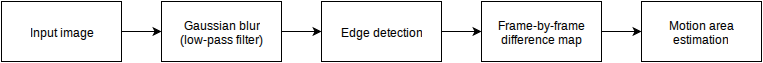
\includegraphics[width=0.8\textwidth]{high_level_block_diagram.png}
	\caption{High-level block diagram describing our implementation of a real-time edge-based motion detector}
	\label{motion-detection-block-diagram}
\end{figure*}


\section{Edge Detection Algorithm}
\label{edge-detection-section}
Edge detection is the process of determining the locations of boundaries that separate objects, or sections of objects, in an image. This edge data simplifies the features of an image to only its basic outlines, which makes it a convenient input for many other problems in computer vision, including motion detection and tracking, object classification, three-dimensional reconstruction, and others. The edge detection algorithm we present is composed of three stages:
\begin{enumerate}
	\item Reduce the amount of high-frequency noise from the image using a two-dimensional low pass filter.
	\item Determine the two-dimensional gradient of the filtered image by applying partial derivatives in both the horizontal and vertical directions.
	\item Classify edges by suppressing surrounding pixels in the gradient direction whose magnitude is lesser, and applying selective thresholding to a limited apron around each selected pixel.
\end{enumerate}
Edges correspond to the points on the image that exhibit a high gradient magnitude. The edge data from our algorithm is then used as input to our motion detection algorithm.

\subsection{Separable Convolution}
The filtering necessary in steps (1) and (2) from our algorithm above involve the convolution of a two-dimensional image and a two-dimensional kernel filter of constant width and height. A na\"{\i}ve implementation of two-dimensional convolution would require a double sum across the kernel and image for each individual pixel:
\begin{equation}
	\label{2d-naive-convolution}
	y[m, n] = x[m, n] * h[m, n] = \sum_{i = -\infty}^{\infty} \sum_{j = -\infty}^{\infty} h[i, j] x[m - i, n - j]
\end{equation}
For an image of size $M \times N$ and kernel of size $k$, a direct implementation would require $O(MNk^2)$ time, which is infeasible for a real-time implementation. Instead, it is possible to exploit the separable property of certain convolution matrices $h$, e.g. that $h$ can be represented as the product of two one-dimensional matrices $h_1$ and $h_2$. This effectively reduces our two-dimensional convolution of Equation \eqref{2d-naive-convolution} to two separate instances of one-dimensional convolution:
\begin{equation}
	\label{separable-convolution-definition}
	y[m, n] = h_1[n] * (h_2[m] * x[m, n])
\end{equation}
which is implemented as
\begin{equation}
	\label{separable-convolution-formula}
	y[m, n] = \sum_{i = -\infty}^{\infty}h_1[i] \sum_{j = -\infty}^{\infty}h_2[j] x[m - i, n - j]
\end{equation}
For the same $M \times N$ input and square kernel of size $k$, a separable implementation reduces the computational complexity to $O(MNk)$. By comparison, an implementation using the FFT would cost $O(MN\log{MN})$. In practice, consider the separable convolution speed gain evident in the following results\footnote{Results were obtained by measuring the CPU execution time of the convolution algorithms implemented in C on an Intel Core i7 4790K @ 4.7 GHz.} for a convolution of a $3 \times 3$ Gaussian filter kernel with images of varying sizes (visualized in Figure \ref{direct-separated-convolution-graph}).
\begin{table}[H]
	\small
	\centering
	\caption{Execution Time of Direct 2D Convolution, $O(MNk^2)$}
	\label{convolution-complexity-comparison}
	\begin{tabular}{llll}
	 Image dimensions & Pixel count ($\times10^6$) & Execution time (s) \\
	 $100 \times 100$ & $0.01$ & $0.000489$ \\
	 $500 \times 500$ & $0.25$ & $0.008784$ \\
	 $1000 \times 1000$ & $1.00$ & $0.034249$ \\
	 $1500 \times 1500$ & $2.25$ & $0.076803$ \\
	 $2000 \times 2000$ & $4.00$ & $0.136222$ \\
	 $2500 \times 2500$ & $6.25$ & $0.212414$ \\
	\end{tabular}
\end{table}
\begin{table}[H]
	\small
	\centering
	\caption{Execution Time of Separated 2D Convolution, $O(MNk)$}
	\label{convolution-complexity-comparison}
	\begin{tabular}{llll}
	 Image dimensions & Pixel count ($\times10^6$) & Execution time (s) \\
	 $100 \times 100$ & $0.01$ & $0.000279$ \\
	 $500 \times 500$ & $0.25$ & $0.004768$ \\
	 $1000 \times 1000$ & $1.00$ & $0.018969$ \\
	 $1500 \times 1500$ & $2.25$ & $0.042410$ \\
	 $2000 \times 2000$ & $4.00$ & $0.075280$ \\
	 $2500 \times 2500$ & $6.25$ & $0.117134$ \\
	\end{tabular}
\end{table}
\begin{figure}
	\centering
	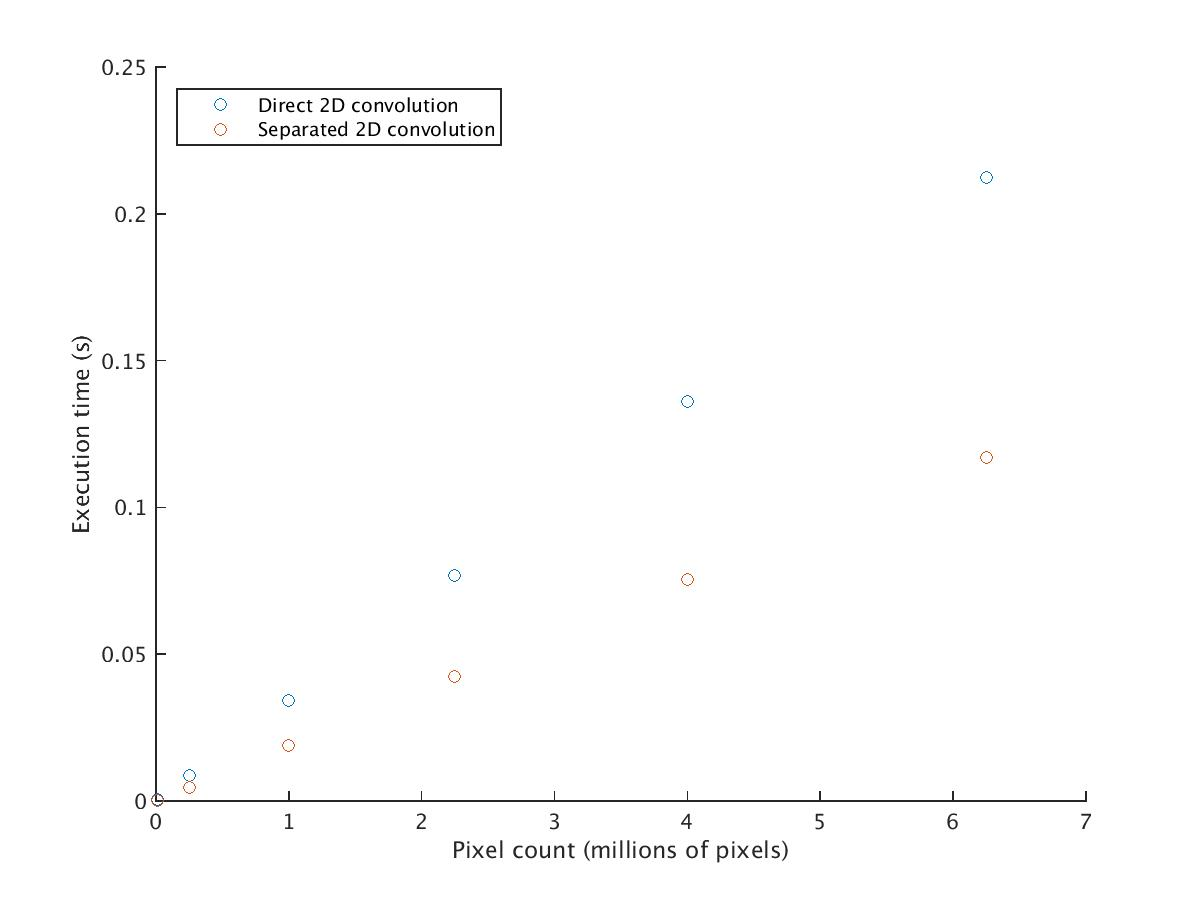
\includegraphics[width=0.45\textwidth]{naive_separable_convolution_execution_time.jpg}
	\caption{Graphical comparison of execution times of direct and separated 2D convolution as a function of the input pixel count}
    \label{direct-separated-convolution-graph}
\end{figure}
As detailed in later sections, we take advantage of the fast computational complexity of separable convolution in our implementation, as all of the filters we apply are separable into one-dimensional matrices.


\subsection{Noise Elimination: Two-Dimensional Gaussian Filtering}
The first task in our edge detection algorithm is denoising the input in order to reduce the amount of high-frequency content in the image by as much as possible without destroying critical information points in the image (e.g. the real edges). We filter out high-frequency noise so that random noise is not mistakenly interpreted as an edge, as edges correspond to points in the image where the gradient has an above-threshold magnitude. \par
For example, consider the $5312 \times 2988$ pixel image (taken at a high ISO to deliberately introduce noise) of Figure \ref{noisy-image} and a plot of its grayscale intensity versus the image's spatial dimensions in Figure \ref{noisy-image-mesh}. It is clear from the mesh that there is much high-frequency noise, which can be removed with a low-pass filter.
\begin{figure}[H]
	\centering
	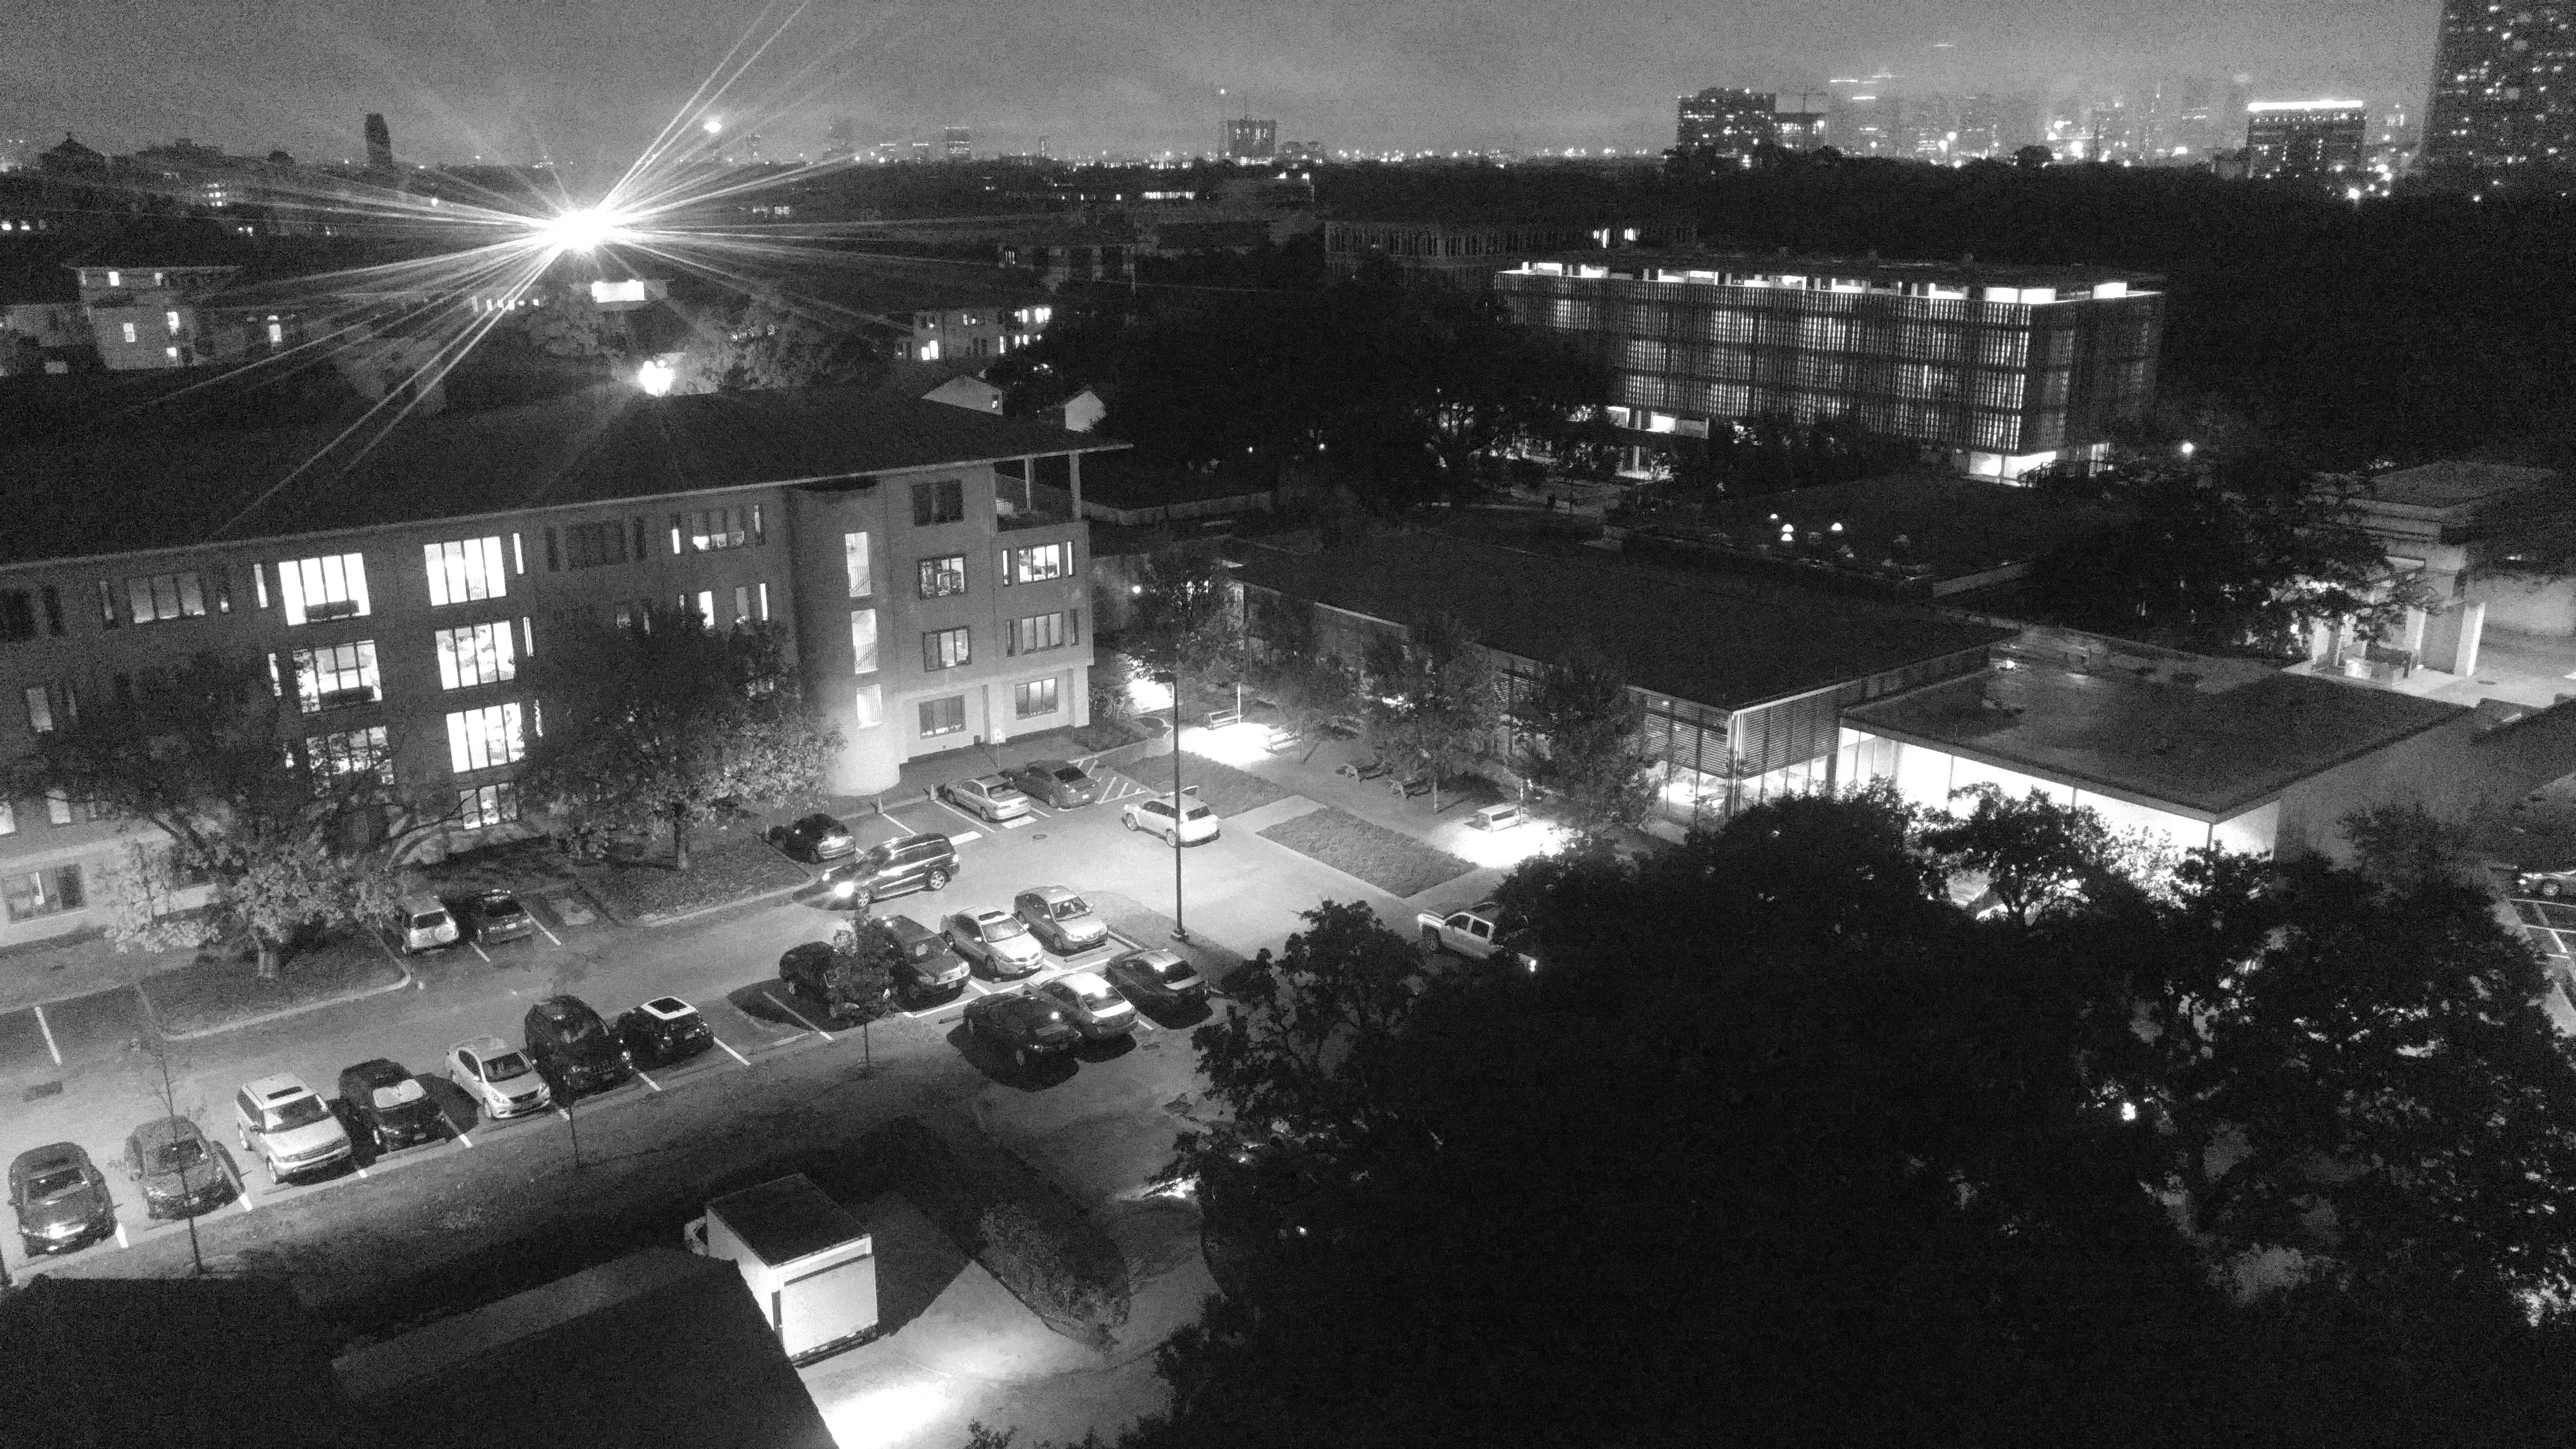
\includegraphics[width=0.45\textwidth]{noisy_image.jpg}
	\caption{Unfiltered noisy image}
    \label{noisy-image}
\end{figure}
\begin{figure}[h]
	\centering
	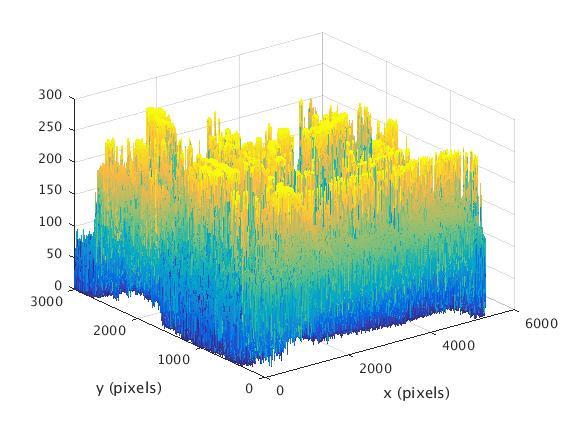
\includegraphics[width=0.45\textwidth]{noisy_image_mesh.jpg}
	\caption{Grayscale intensity of unfiltered noisy image at each pixel}
    \label{noisy-image-mesh}
\end{figure}
\begin{figure}[h]
	\centering
	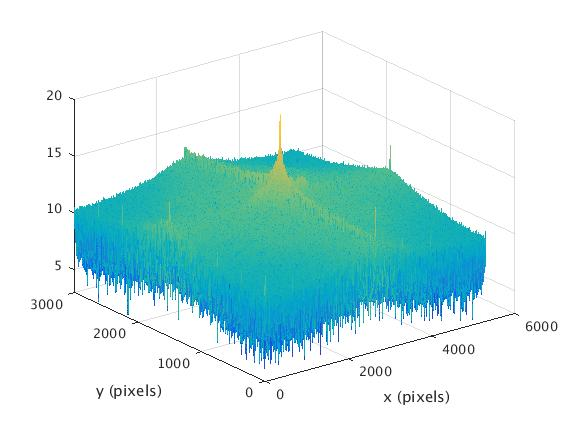
\includegraphics[width=0.45\textwidth]{fft_noisy_image.jpg}
	\caption{FFT magnitude of unfiltered noisy image at each pixel (log scale)}
    \label{noisy-image-fft}
\end{figure}
To low-pass filter our image, we apply a discrete Gaussian filter. Generally, a Gaussian blur kernel of size $2n + 1 \times 2n + 1$ ($\forall n \in \mathbb{Z}^+$, and with parameter $\sigma$) is given by
$$h[i, j] = \frac{1}{2\pi \sigma^2}e^{-\frac{(i - k - 1)^2 + (j - k - 1)^2}{2\sigma^2}}$$
Our implementation of Gaussian filtering uses the constant-sized ($k = 3$), constant-$\sigma$ kernel
\[
h[i, j] = \frac{1}{16}
\begin{bmatrix}
	1 & 2 & 1 \\
	2 & 4 & 2 \\
	1 & 2 & 1
\end{bmatrix}
\]
This kernel is implemented separably as
\begin{equation}
	\label{gaussian-filter}
	h[i, j] = \frac{1}{16}
	\begin{bmatrix}
		1 & 2 & 1
	\end{bmatrix}
	*
	\begin{bmatrix}
		1 \\ 2 \\ 1
	\end{bmatrix}
\end{equation}
\par Applying a Gaussian filter with parameters $k = 5$ and $\sigma = 5$ to the above image significantly denoises the image without sacrificing edge precision, which can be seen from the spatial intensity plot in Figure \ref{filtered-noisy-image-mesh}.
\begin{figure}[H]
	\centering
	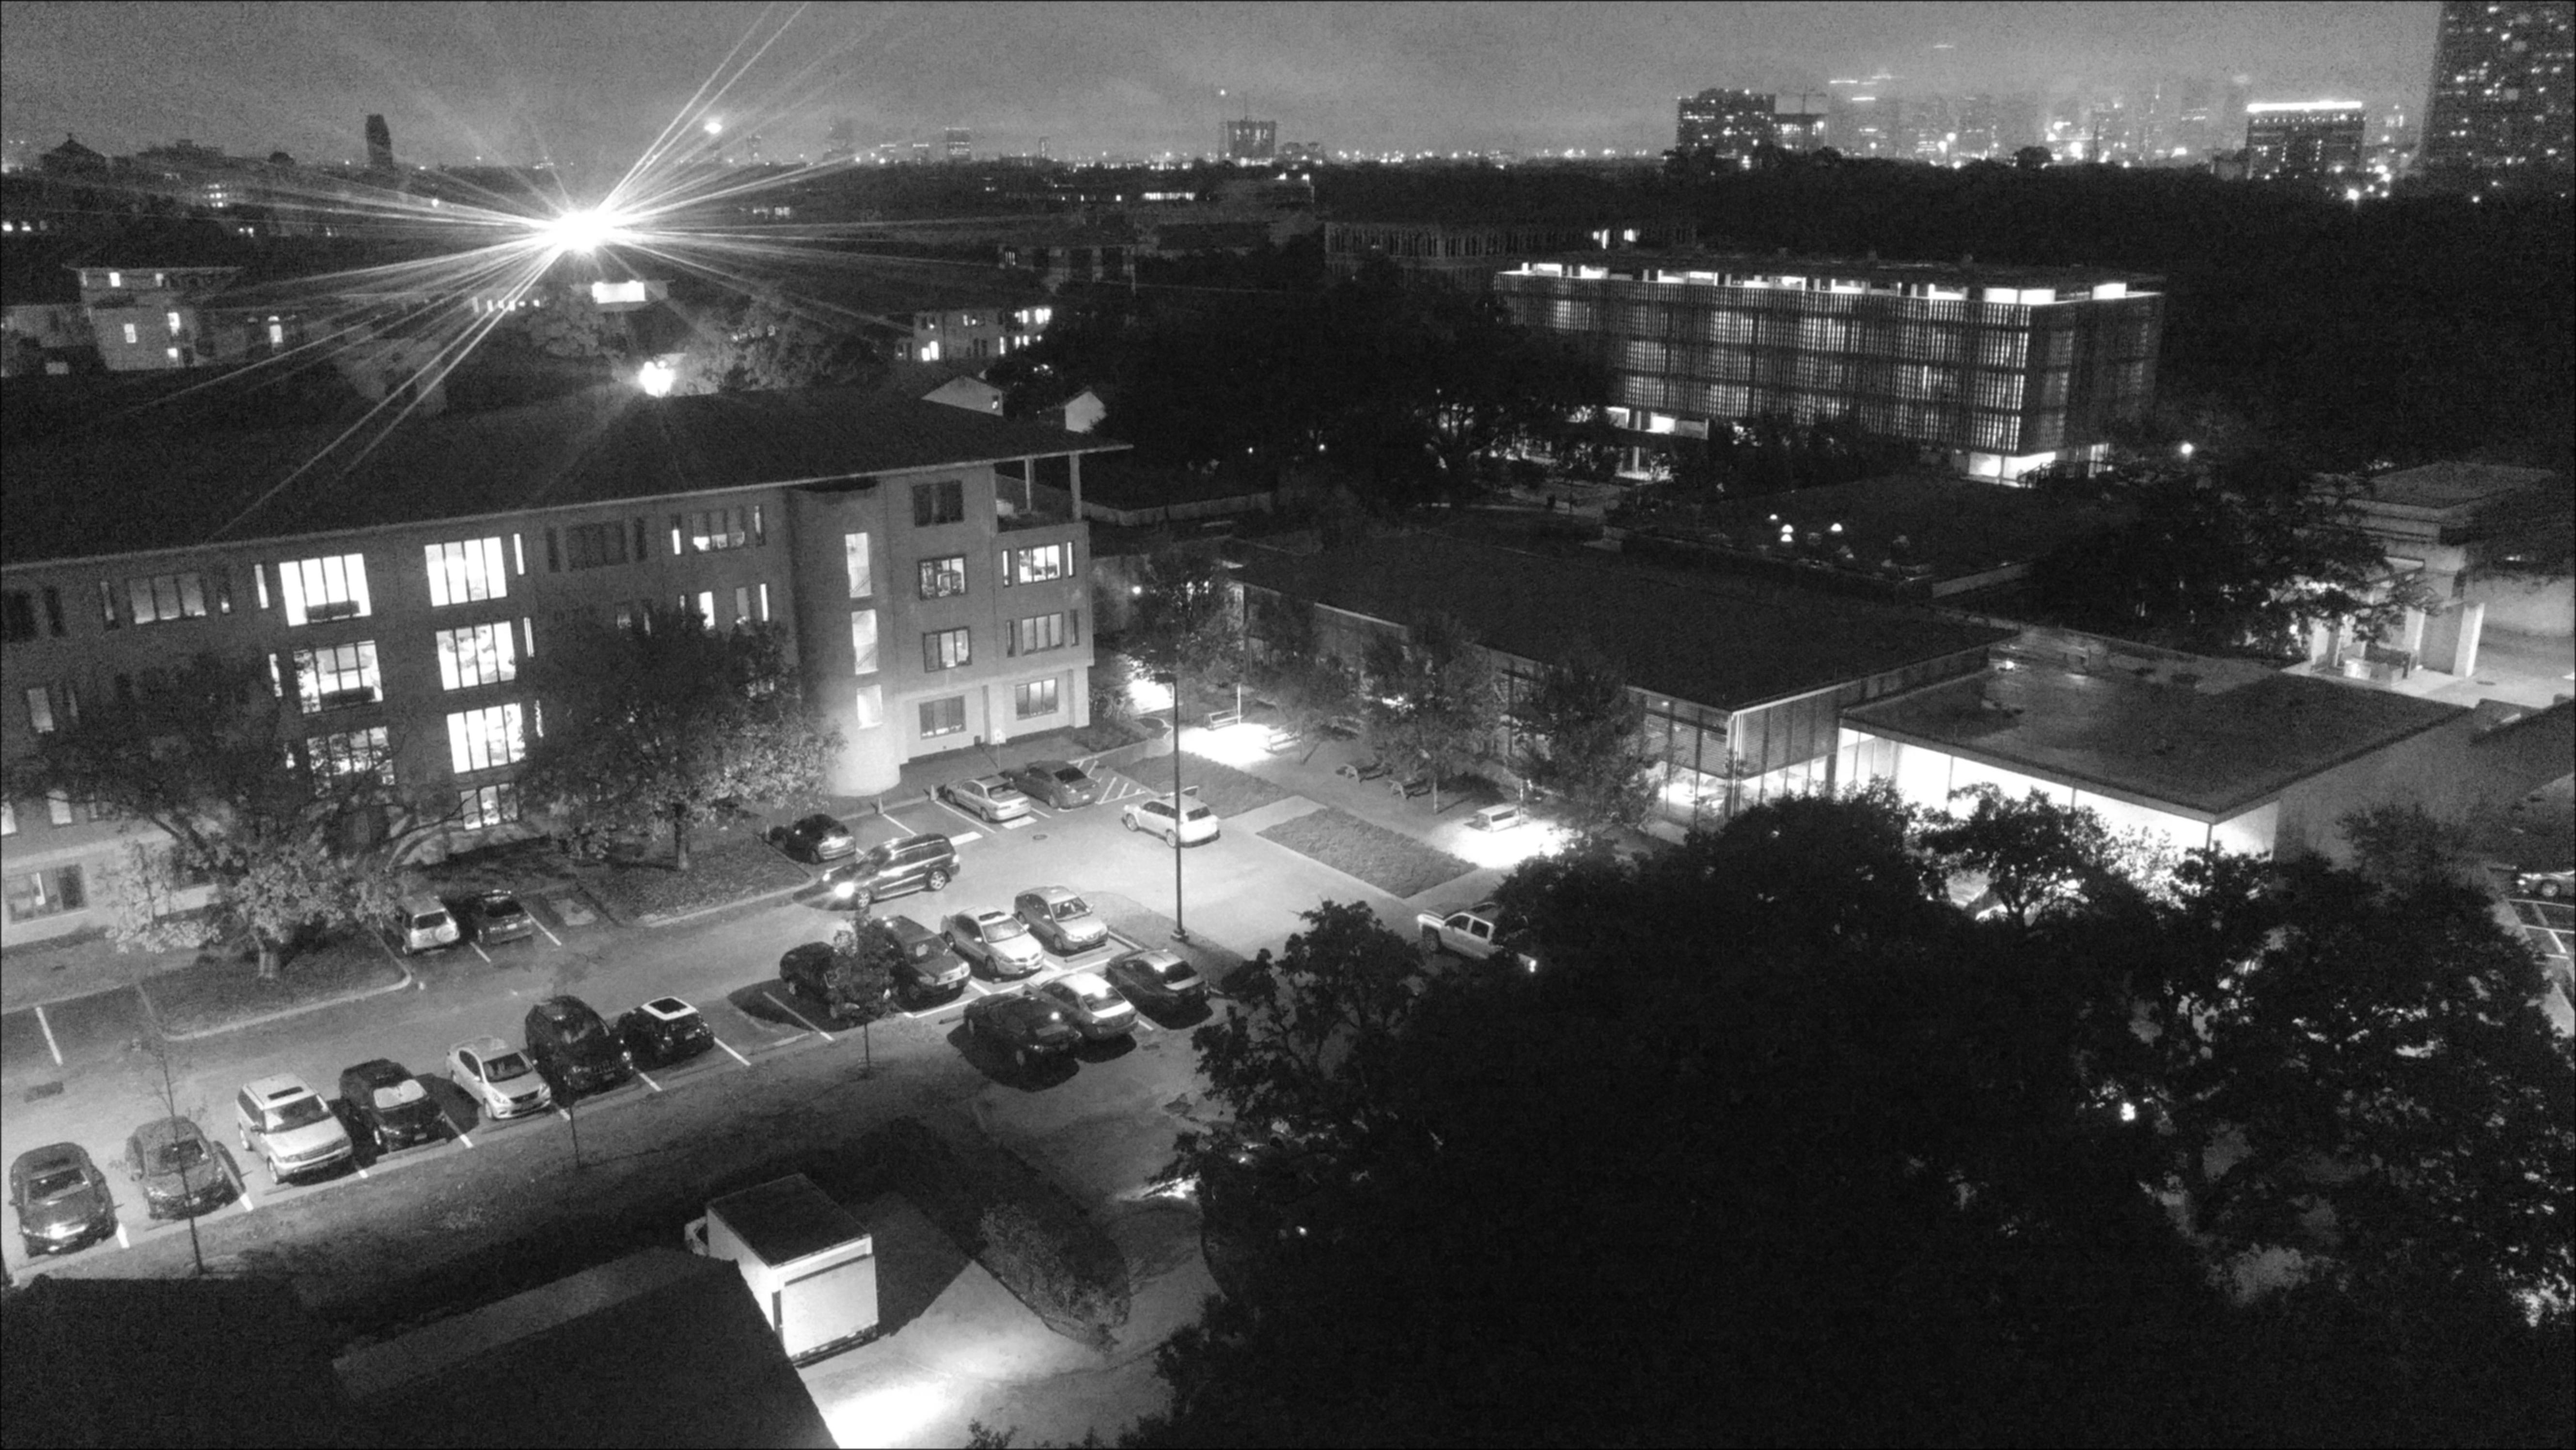
\includegraphics[width=0.45\textwidth]{filtered_noisy_image.jpg}
	\caption{Gaussian-filtered noisy image with parameters $k = 3$ and $\sigma = 5$}
    \label{filtered-noisy-image}
\end{figure}
\begin{figure}[h]
	\centering
	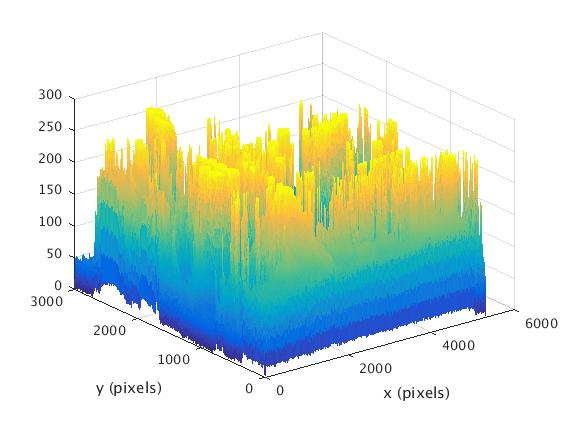
\includegraphics[width=0.45\textwidth]{filtered_noisy_image_mesh.jpg}
	\caption{Grayscale intensity of Gaussian-filtered noisy image at each pixel}
    \label{filtered-noisy-image-mesh}
\end{figure}
\begin{figure}[h]
	\centering
	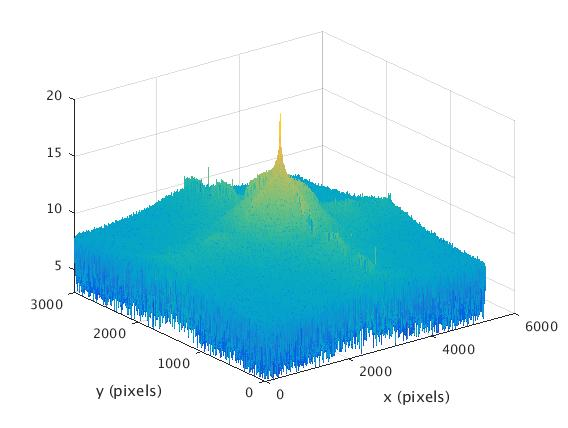
\includegraphics[width=0.45\textwidth]{fft_filtered_noisy_image.jpg}
	\caption{FFT magnitude of Gaussian-filtered noisy image at each pixel (log scale)}
    \label{filtered-noisy-image-fft}
\end{figure}

\subsection{Gradient Computation: The Sobel Operator}
Edges in the image correspond to pixel locations at which there is a rapid change in intensity with respect to the image's spatial dimensions. Thus, edge pixels are defined as those whose gradient magnitude $||\boldsymbol{G}||$ is maximized along the gradient direction $\theta_G$.
\begin{equation}
	\label{gradient-magnitude}
	||\boldsymbol{G}_{i,j}|| = \sqrt{G_x^2 + G_y^2}
\end{equation}
\begin{equation}
	\label{gradient-angle}
	\theta_G = \arctan{\frac{G_y}{G_x}}
\end{equation}
where $G_x$ and $G_y$ are the values of the partial derivatives along the $x$ and $y$ directions, respectively, at the pixel located at $(i, j)$ of the image $A$.
$$G_x = \frac{\partial \boldsymbol{A}}{\partial x}\Bigr|_{\substack{(x, y) = (i, j)}}$$
$$G_y = \frac{\partial \boldsymbol{A}}{\partial y}\Bigr|_{\substack{(x, y) = (i, j)}}$$
\par A variety of different discrete differentiation operators exist to approximate the gradient of the image. The operator we choose in our implementation is the Sobel operator.
\[
\boldsymbol{G_x} =
\begin{bmatrix}
	-1 & 0 & 1 \\
	-2 & 0 & 2 \\
	-1 & 0 & 1
\end{bmatrix} * \boldsymbol{A}
\]
\[
\boldsymbol{G_y} =
\begin{bmatrix}
	-1 & -2 & -1 \\
	0 & 0 & 0 \\
	1 & 2 & 1
\end{bmatrix} * \boldsymbol{A}
\]
Like our Gaussian kernel, the Sobel operator (in both the $x$ and $y$ directions) is separable:
\begin{equation}
	\label{horizontal-sobel-filter}
	\boldsymbol{G_x} =
	\begin{bmatrix}
		1 \\
		2 \\
		1
	\end{bmatrix} * 
	(\begin{bmatrix}
		1 & 0 & -1
	\end{bmatrix} * \boldsymbol{A})
\end{equation}
\begin{equation}
	\label{vertical-sobel-filter}
	\boldsymbol{G_y} =
	\begin{bmatrix}
		1 \\
		0 \\
		-1
	\end{bmatrix} * 
	(\begin{bmatrix}
		1 & 2 & 1
	\end{bmatrix} * \boldsymbol{A})
\end{equation}
\par Thus, we perform two separable convolutions with the separated Sobel filter on the Gaussian-filtered image to obtain gradients in the horizontal and vertical directions, and determine the magnitude and angle matrices $\boldsymbol{G}$ and $\boldsymbol{\theta}$ from equations \eqref{gradient-magnitude} and \eqref{gradient-angle}.
\begin{figure}[h]
	\centering
	\includegraphics[width=0.45\textwidth]{pcb.jpg}
	\caption{Original image input to Sobel filter}
    \label{pcb-original}
\end{figure}
\begin{figure}[h]
	\centering
	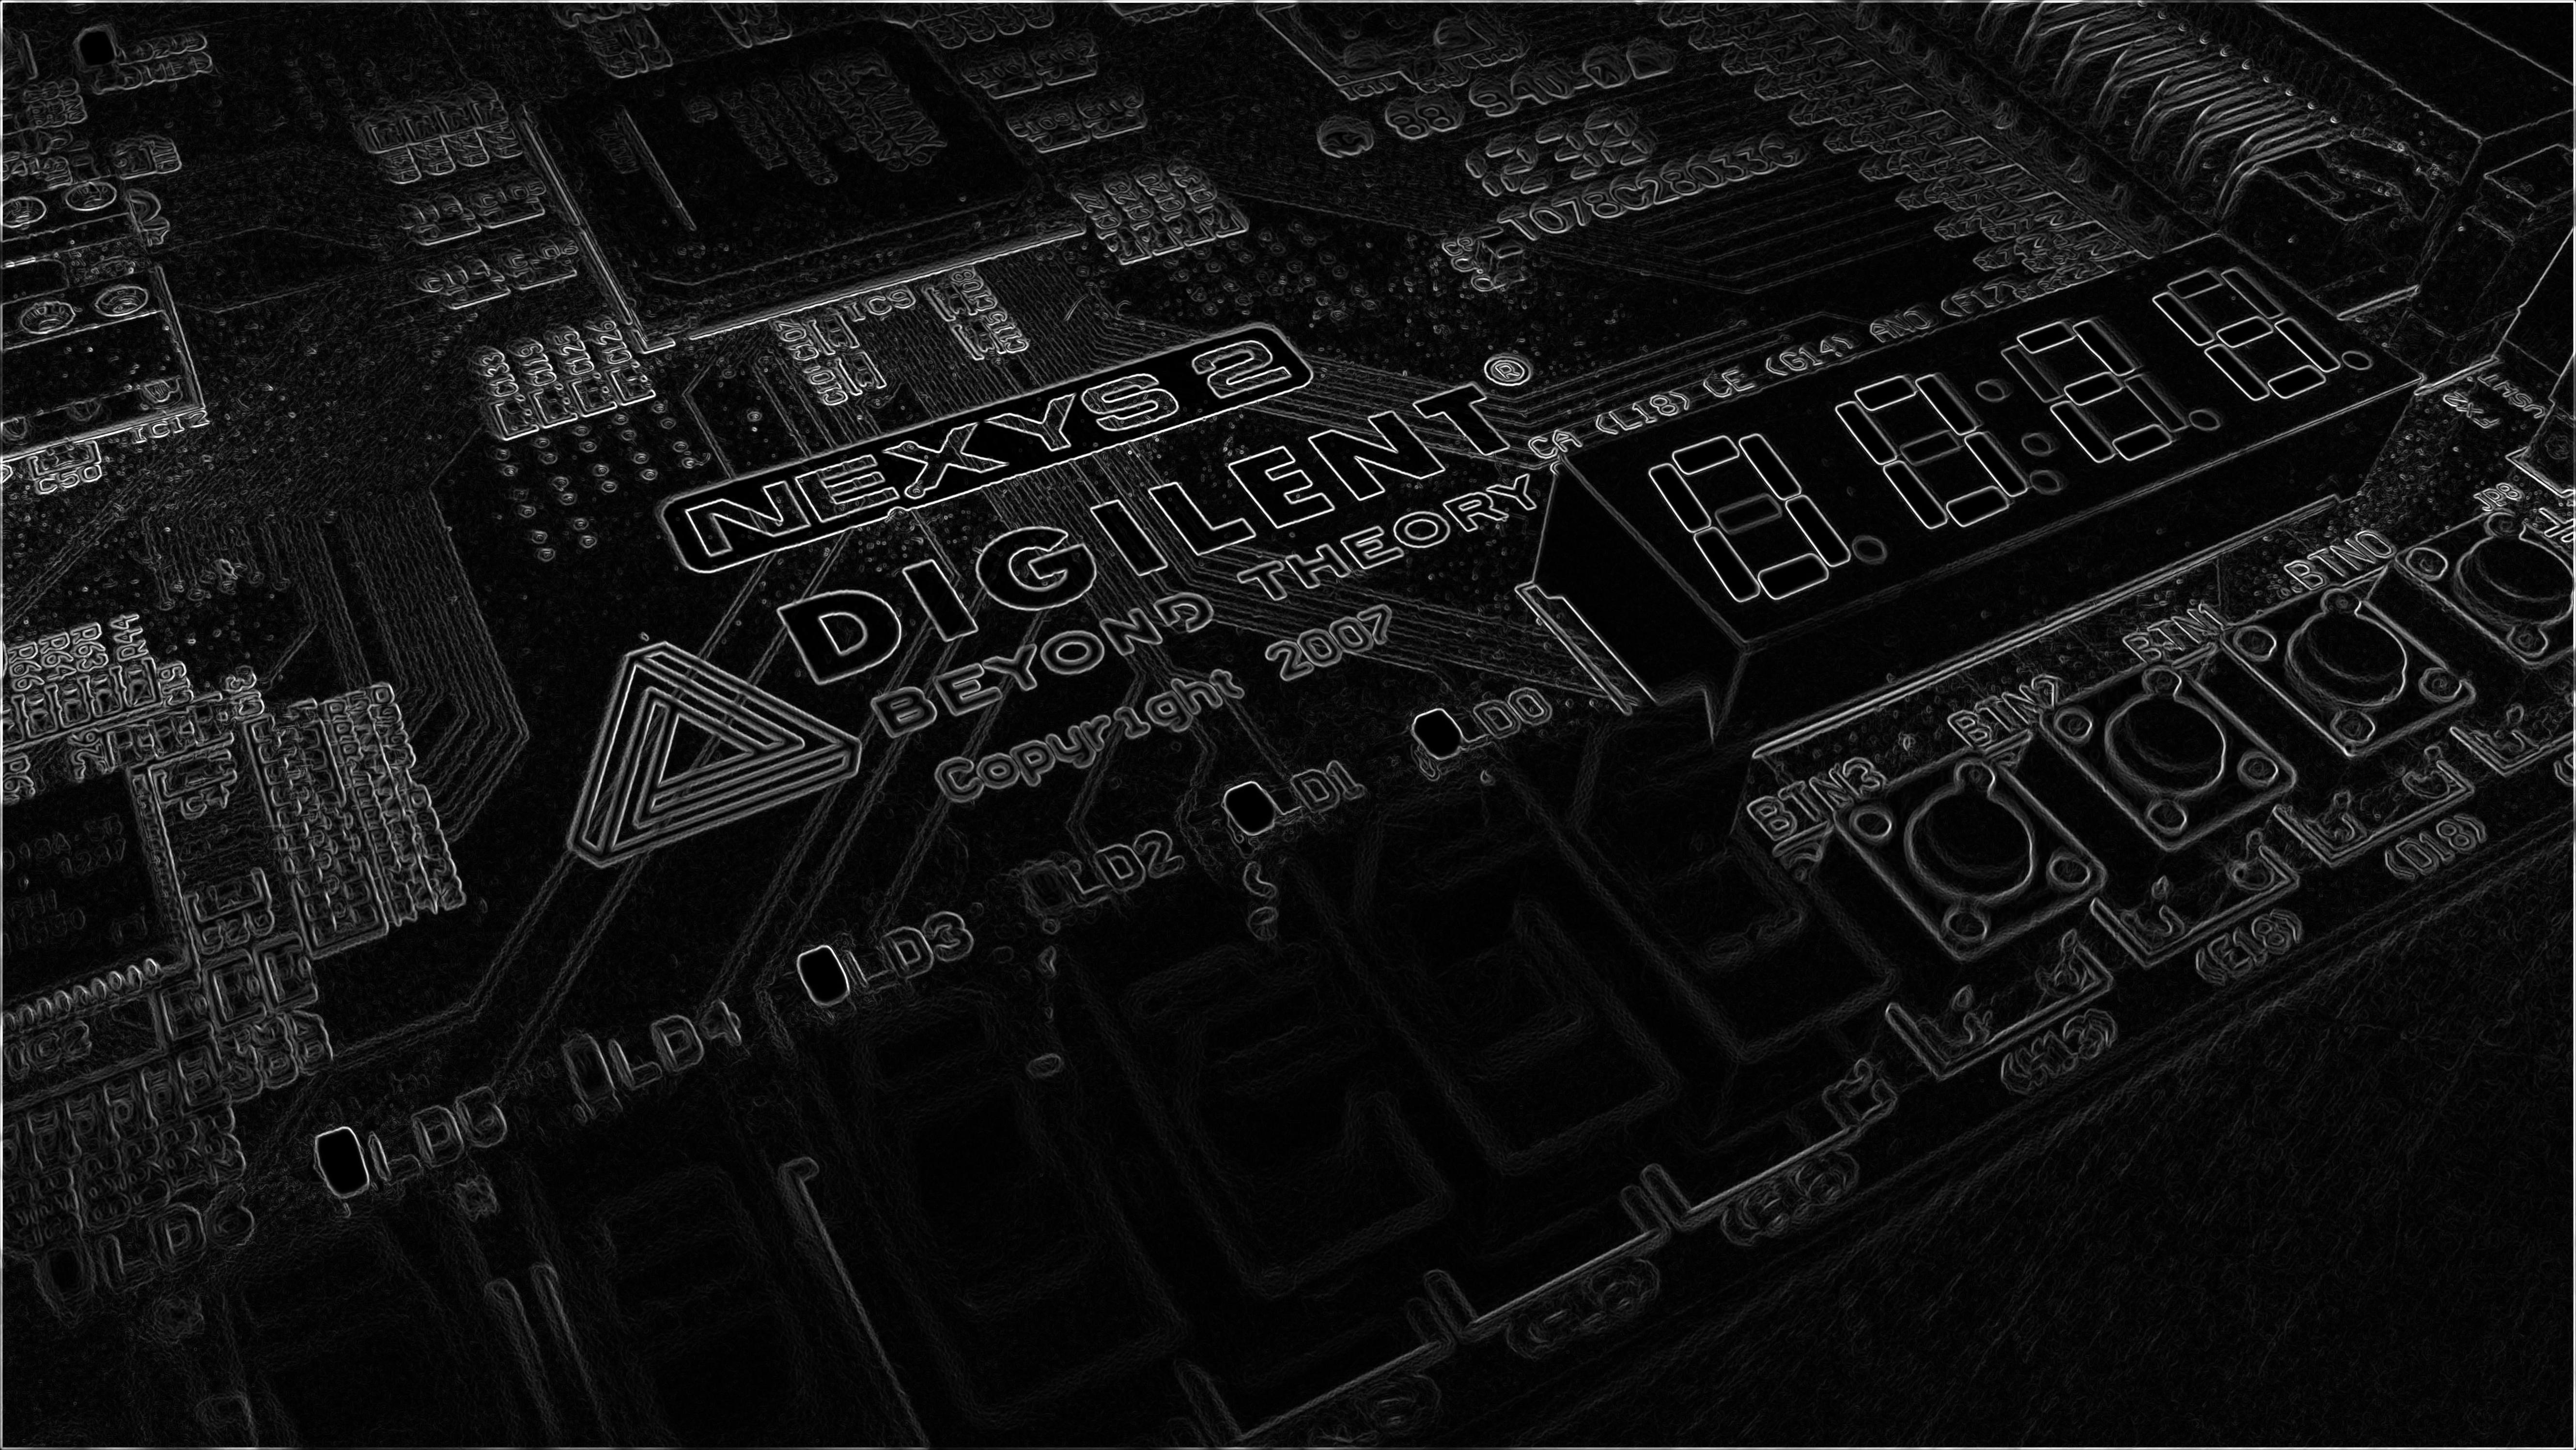
\includegraphics[width=0.45\textwidth]{sobel_pcb.jpg}
	\caption{Magnitude of the gradient $||\boldsymbol{G}||$, as determined by applying a Sobel filter in both the $x$ and $y$ directions, at each pixel of the Gaussian-filtered original image with parameters $k = 5$ and $\sigma = 5$}
    \label{sobel-pcb}
\end{figure}
\begin{figure}[h]
	\centering
	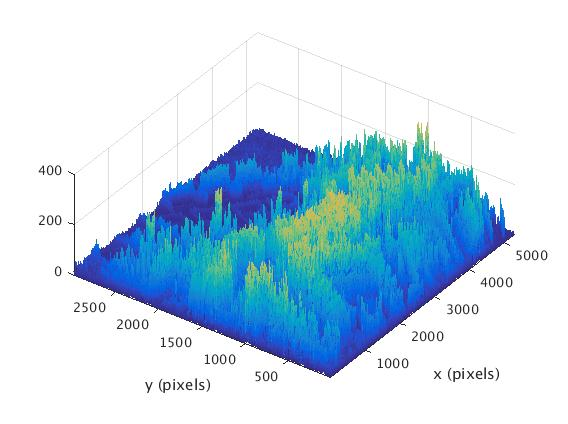
\includegraphics[width=0.45\textwidth]{sobel_pcb_mesh.jpg}
	\caption{Gradient of Figure \ref{sobel-pcb} visualized as a three-dimensional mesh}
    \label{sobel-pcb-mesh}
\end{figure}

\subsection{Non-Maximum Suppression and Selective Thresholding}
Given the gradient magnitude and direction of the Gaussian-filtered image, the final step of the edge detection algorithm is to determine which pixels should be selected as edge pixels, and which should be rejected. We define two procedures, \textit{non-maximum suppression} and \textit{selective thresholding}, to gain a reasonably accurate edge map from the gradient.
\par Non-maximum suppression selects and rejects edge pixels according to the following criteria:
\begin{enumerate}
	\item Pixels whose gradient magnitude is below a user-defined low threshold, $t_l$, is immediately rejected
	\item If the gradient magnitude of a pixel is greater than that of the pixels in either direction of the gradient angle of that pixel, then the pixel is accepted if its gradient magnitude is greater than a user-defined high threshold, $t_h$
\end{enumerate}
More precisely, a pixel at $(i, j)$ with gradient magnitude $G_{i, j} > t_l$ and angle $\theta$ is accepted if any of the following hold true:
\begin{itemize}
	\item $(-\frac{\pi}{6} < \theta < \frac{\pi}{6} \vee -\pi < \theta < -\frac{5 \pi}{6} \vee \frac{5\pi}{6} < \theta < \pi) \wedge G_{i, j} > G_{i, j \pm 1}$
	\item $(\frac{\pi}{6} < \theta < \frac{\pi}{3} \vee -\frac{5 \pi}{6} < \theta < -\frac{2 \pi}{3}) \wedge G_{i, j} > G_{i \pm 1, \pm j}$
	\item $(\frac{\pi}{3} < \theta < \frac{2 \pi}{3} \vee -\frac{2 \pi}{3} < \theta < -\frac{\pi}{3}) \wedge G_{i, j} > G_{i \pm 1, j}$
	\item $(\frac{2 \pi}{3} < \theta < \frac{5 \pi}{6} \vee -\frac{\pi}{3} < \theta < -\frac{\pi}{6}) \wedge G_{i, j} > G_{i \pm 1, \mp j}$
\end{itemize}
The selective thresholding technique extends on the procedure of non-maximum suppression. For any pixel that passes criteria (2) (maximized, relative to the neighboring pixels, along the gradient direction), consider an $\alpha$ x $\alpha$ box around the pixel. If any pixel within the box exceeds the low threshold $t_l$, then the pixel is accepted. This technique attempts to catch pixels that might ``connect" ridge pixels identified by criteria (2) but fail to satisfy the criterion themselves, in order to create more continuous edge lines.
\begin{figure}[]
	\centering
	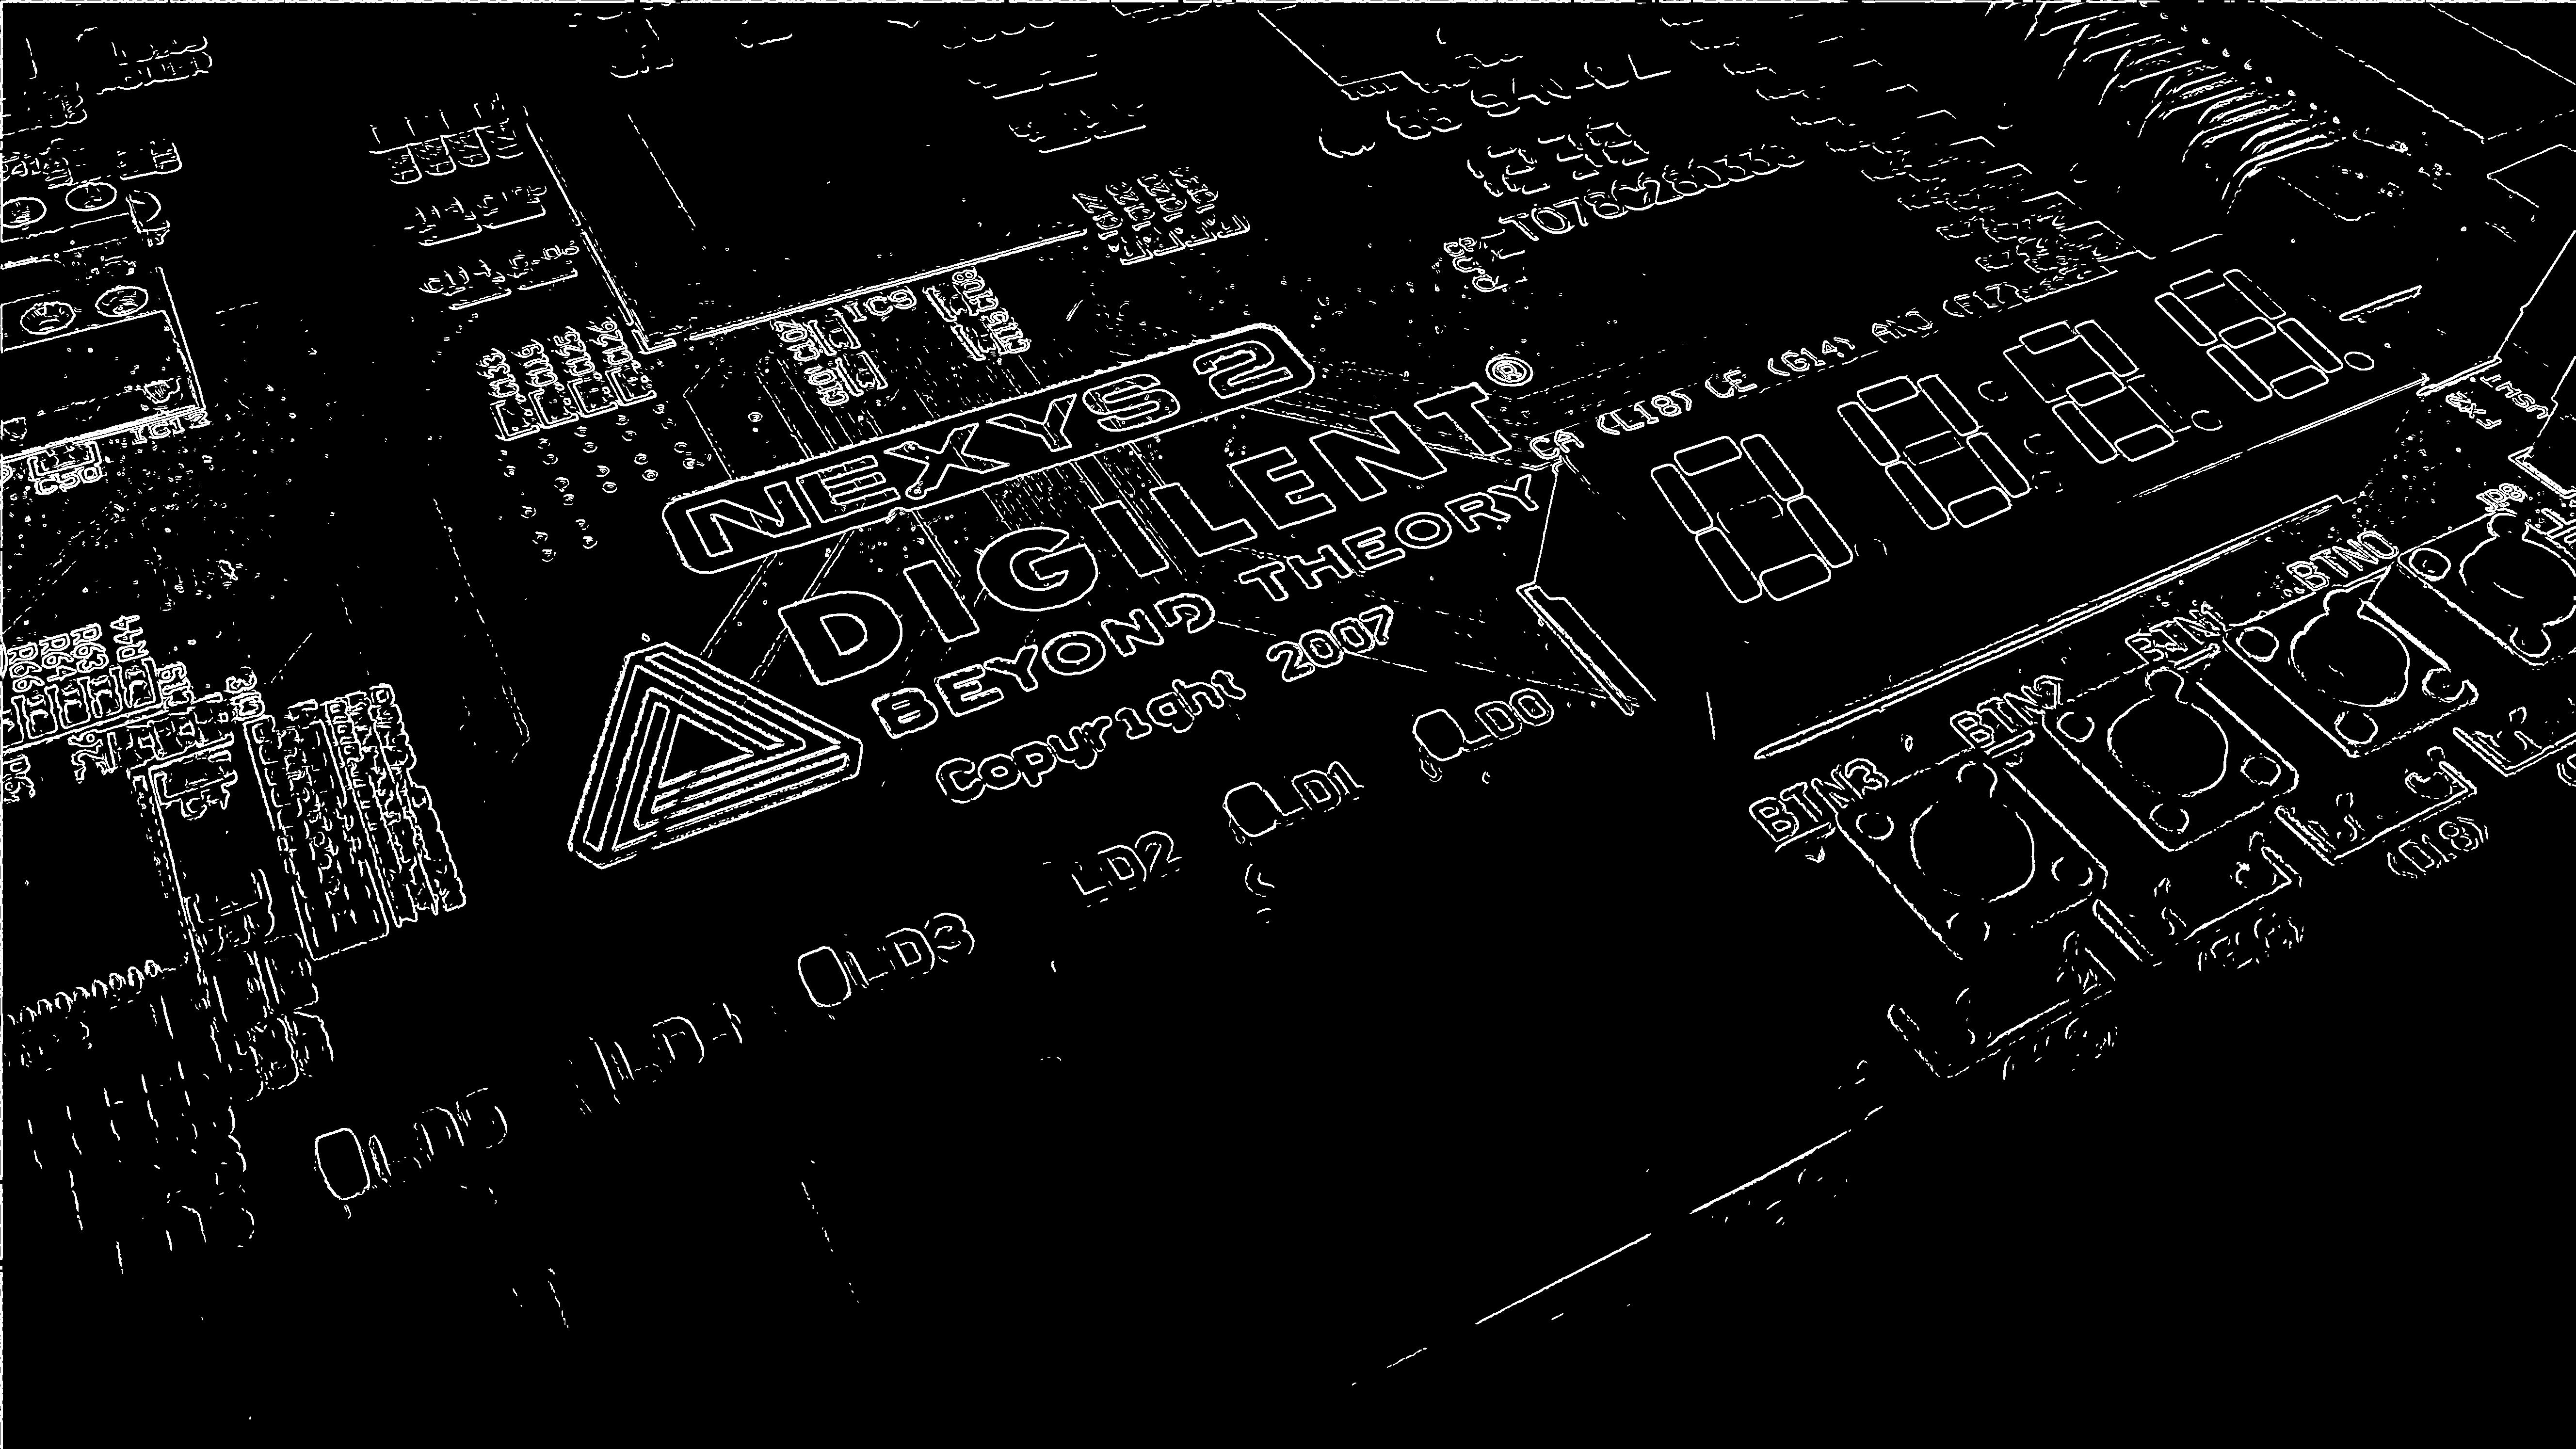
\includegraphics[width=0.45\textwidth]{pcb_edges.jpg}
	\caption{Output of edge detection algorithm after non-maximum suppression and selective thresholding on the image of Figure \ref{pcb-original}, with parameters $t_l = 70$ and $t_h = 80$}
    \label{pcb-edges}
\end{figure}
\begin{algorithm}[h]
	\smaller
	\label{non-maximum-suppression-selective-thresholding-algorithm}
	\caption{Non-maximum suppression and selective thresholding: pseudocode for a serial, CPU implementation}
	
	\KwIn{Gradient magnitude matrix $\boldsymbol{G}_{i, j}$ and gradient angle matrix $\boldsymbol{\theta}_{i, j}$ for an image $\boldsymbol{A}_{i, j}$, $\forall i \in [0, M - 1], \forall j \in [0, N - 1]$, $\alpha$ (representing the size of the box around which to apply selective thresholding), $t_h$ (the high threshold), and $t_l$ (the low threshold)}
	\KwOut{Edge matrix $\boldsymbol{E}$ of dimensions $M \times N$ that represent the edges of $\boldsymbol{A}$; any entry $\boldsymbol{E}_{i, j}$ is $255$ if an edge is present, and $0$ if an edge is not present}
	
	\nl Initialize $\boldsymbol{E}$ to 0 $\forall i \in [0, M - 1], \forall j \in [0, N - 1]$\;
	\nl \ForEach {$i \in [\alpha + 1, M - \alpha - 2]$} {
		\nl \ForEach {$j \in [\alpha + 1, N - \alpha - 2]$} {
			\nl HorizontalGradient $\gets -\frac{\pi}{6} < \boldsymbol{\theta}_{i, j} < \frac{\pi}{6} \vee -\pi < \boldsymbol{\theta}_{i, j} < -\frac{5 \pi}{6} \vee \frac{5\pi}{6} < \boldsymbol{\theta}_{i, j} < \pi$\;
			\nl HorizontalMax $\gets$ HorizontalGradient $\wedge \boldsymbol{G}_{i, j} > \boldsymbol{G}_{i, j \pm 1}$\;
			\nl PosDiagonalGradient $\gets \frac{\pi}{6} < \boldsymbol{\theta}_{i, j} < \frac{\pi}{3} \vee -\frac{5 \pi}{6} < \boldsymbol{\theta}_{i, j} < -\frac{2 \pi}{3}$\;
			\nl PosDiagonalMax $\gets$ PosDiagonalGradient $\wedge \boldsymbol{G}_{i, j} > \boldsymbol{G}_{i \pm 1, \pm j}$\;
			\nl VerticalGradient $\gets \frac{\pi}{3} < \boldsymbol{\theta}_{i, j} < \frac{2 \pi}{3} \vee -\frac{2 \pi}{3} < \boldsymbol{\theta}_{i, j} < -\frac{\pi}{3}$\;
			\nl VerticalMax $\gets$ VerticalGradient $\wedge \boldsymbol{G}_{i, j} > \boldsymbol{G}_{i \pm 1, j}$\;
			\nl NegDiagonalGradient $\gets \frac{2 \pi}{3} < \boldsymbol{\theta}_{i, j} < \frac{5 \pi}{6} \vee -\frac{\pi}{3} < \boldsymbol{\theta}_{i, j} < -\frac{\pi}{6}$\;
			\nl NegDiagonalMax $\gets$ NegDiagonalGradient $\wedge \boldsymbol{G}_{i, j} > \boldsymbol{G}_{i \pm 1, \mp j}$\;
			
			\nl \If {$\boldsymbol{G}_{i, j} > t_h \wedge ($\textnormal{HorizontalMax} $\vee$ \textnormal{PosDiagonalMax} $\vee$ \textnormal{VerticalMax} $\vee$ \textnormal{NegDiagonalMax}$)$} {
				\ForEach {$i' \in [-\alpha, \alpha]$} {
					\ForEach {$j' \in [-\alpha, \alpha]$} {
						\nl \If{$\boldsymbol{G}_{i + i', j + j'} > t_l$} {
							\nl $\boldsymbol{E}_{i + i', j + j'} \gets 255$\;
						}
					}
				}
			}
		}
	}
	\nl \Return $\boldsymbol{E}$\;
	\
\end{algorithm}

\subsection{GPU Parallelization and CUDA Implementation}
We begin with a parallelized implementation of separable convolution, since the same convolution operation is applied for both the initial Gaussian low pass filter and the edge detecting Sobel filter. Our parallel implementation involves first independently computing the convolution with the horizontal filter ($h_2$ in Equation \eqref{separable-convolution-definition}), then convolving that result with the vertical filter $h_1$. In computing the output $y[m, n]$ at every index $(i, j)$, we launch a kernel with 16 threads per block, where the total number of blocks along one dimension is equal to the size of that dimension divided by 16. For our 5312 x 2988 test images, this corresponds to 332 blocks in the horizontal direction and 186 blocks in the vertical direction, each with 16 computational threads.
\begin{lstlisting}[
	caption=Grid configuration for the separable convolution device kernel,
	label=grid-configuration,
	language=C
]
#define TX 16
#define TY 16

dim3 block_size(TX, TY);
int bx_horizontal = horizontal_convolution_width/block_size.x;
int by_horizontal = horizontal_convolution_height/block_size.y;
dim3 grid_size_horizontal = dim3(bx_horizontal, by_horizontal);
int bx_vertical = vertical_convolution_width/block_size.x;
int by_vertical = vertical_convolution_height/block_size.y;
dim3 grid_size_vertical = dim3(bx_vertical, by_vertical);

horizontal_convolve<<<grid_size_horizontal, block_size>>>(...);
vertical_convolve<<<grid_size_vertical, block_size>>>(...);
\end{lstlisting}
\par The convolution on the device executes only one serial loop across the dimensions of the filter exactly as it is defined in Equation \eqref{separable-convolution-formula}. This sum is then stored in the output array\footnote{In our implementation, we represent a two-dimensional image as a one-dimensional array by directly concatenating the rows of the matrix into a single array. Thus, for a matrix of size $M \times N$, the index $(i, j)$ would correspond to index $Ni + j$ in our one-dimensional array.} according to the block index, block size, and thread index. The implementation is modularized so that any separable filter can be applied to an input matrix.
\begin{lstlisting}[
	caption=Implementation of horizontal and vertical separated convolution,
	label=separable-convolution-implementation,
	language=C
]
__global__ void horizontal_convolve(int *d_out, int *x, int *h, int x_width, int x_height, int h_width, int h_height) {
    const int r = blockIdx.y * blockDim.y + threadIdx.y;
    const int c = blockIdx.x * blockDim.x + threadIdx.x;
    const int i = r * (x_width + h_width - 1) + c;
    
    int sum = 0;
    for (int j = 0; j < h_width; j++) {
        int p = x_width*r + c - j;
        if (c - j >= 0 && c - j < x_width) {
            sum += h[j] * x[p];
        }
    }
    d_out[i] = sum;
    __syncthreads();
}

__global__ void vertical_convolve(int *d_out, int *x, int *h, int x_width, int x_height, int h_width, int h_height, double constant_scalar) {
	const int r = blockIdx.y * blockDim.y + threadIdx.y;
	const int c = blockIdx.x * blockDim.x + threadIdx.x;
	const int i = r * x_width + c;

    int sum = 0;
    for (int j = 0; j < h_height; j++) {
        int p = x_width*(r - j) + c;
        if (r - j >= 0 && r - j < x_height) {
            sum += h[j] * x[p];
        }
    }
    d_out[i] = (int)(constant_scalar * (double)sum);
    __syncthreads();
}
\end{lstlisting}
\par The first stage of our edge detection algorithm uses the separable convolution GPU implementation above to apply a Gaussian low-pass filter in Equation \ref{gaussian-filter} to remove high-frequency noise from the image that might be falsely labeled as an edge. Then, the same separable convolution kernel is used to apply the Sobel edge filter of Equations \ref{horizontal-sobel-filter} and \ref{vertical-sobel-filter} to the Gaussian low pass-filtered image in both the horizontal and vertical directions to approximate the horizontal and vertical partial derivatives, respectively. In order to reduce redundancy in computation, the final stage of non-maximum suppression and selective thresholding is separated into two tasks, each of which is implemented in parallel:
\begin{enumerate}
	\item Calculate the gradient magnitude matrix $\boldsymbol{G}$ and gradient angle matrix $\boldsymbol{\theta}$
	\item Implement Algorithm \ref{non-maximum-suppression-selective-thresholding-algorithm} with the inputs $\boldsymbol{G}$ and $\boldsymbol{\theta}$ calculated above
\end{enumerate}
\begin{lstlisting}[
	caption=GPU computation of gradient magnitude and angle,
	label=gradient-magnitude-angle-implementation,
	language=C
]
__global__ void gradient_magnitude_and_direction(
		double *dev_magnitude_output,
		double *dev_angle_output
		int input_width,
		int input_height,
		int *g_x,
		int *g_y
	) {
	const int r = blockIdx.y * blockDim.y + threadIdx.y;
	const int c = blockIdx.x * blockDim.x + threadIdx.x;
	const int i = r * (input_width + 2) + c;
	
	dev_magnitude_output[i] = sqrt(pow((double)g_x[i], 2) + pow((double)g_y[i], 2));
	dev_angle_output[i] = atan2((double)g_y[i], (double)g_x[i]);
}
\end{lstlisting}
Following completion of the computation of Listing \ref{gradient-magnitude-angle-implementation}, the result is input to our implementation of Algorithm \ref{non-maximum-suppression-selective-thresholding-algorithm}. While each of these two tasks operates in parallel (e.g. that each pixel's magnitude/angle or edge property is computed in parallel with the other pixels), the two tasks themselves execute serially. This is due to the fact that the non-maximum suppression and selective thresholding procedure relies on the gradient and angle at each pixel to have already been computed when the algorithm begins. Nonetheless, despite the fact that such serial separation of tasks reduces redundancies in gradient magnitude/angle computations\footnote{Computational redundancy arises from the fact that the non-maximum suppression and selective thresholding procedure needs access to the magnitude and angle of all the pixels in a box of area $\alpha^2$ centered at the current pixel. Calculating these properties directly for each pixel during the algorithm will result in calculation of the same magnitude and angle for the same pixel multiple times.}, further optimization is possible to reduce the amount of time that any thread is idle (which occurs after a particular pixel's gradient magnitude/angle is computed but before its edge property is computed).
\begin{lstlisting}[
	caption=GPU non-maximum suppression and selective thresholding,
	label=non-maximum-suppression-selective-thresholding-implementation,
	language=C
]
__global__ void thresholding_and_suppression(
	int *dev_output,
	double *dev_magnitude,
	double *dev_angle,
	int input_width,
	int input_height,
	int *g_x,
	int *g_y,
	int high_threshold,
	int low_threshold
) {
	const int r = blockIdx.y * blockDim.y + threadIdx.y;
	const int c = blockIdx.x * blockDim.x + threadIdx.x;
    const int i = r * (input_width + 2) + c;

    // First, initialize the current pixel to zero (non-edge)
    dev_output[i] = 0;
    // Boundary conditions
    if (r > 1 && c > 1 && r < input_height - 1 && c < input_width - 1) {
        double magnitude = dev_magnitude[i];
        if (magnitude > high_threshold) {
        	// Non-maximum suppression: determine magnitudes in the surrounding pixel and the gradient direction of the current pixel
        	double magnitude_above = dev_magnitude[(r - 1) * input_width + c];
			double magnitude_below = dev_magnitude[(r + 1) * input_width + c];
			double magnitude_left = dev_magnitude[r * input_width + c - 1];
			double magnitude_right = dev_magnitude[r * input_width + c + 1];
			double magnitude_upper_right = dev_magnitude[(r + 1) * input_width + c + 1];
			double magnitude_upper_left = dev_magnitude[(r + 1) * input_width + c - 1];
			double magnitude_lower_right = dev_magnitude[(r - 1) * input_width + c + 1];
			double magnitude_lower_left = dev_magnitude[(r - 1) * input_width + c - 1];
			double theta = dev_angle[i];
		
			// Check if the current pixel is a ridge pixel, e.g. maximized in the gradient direction
			int vertical_check = (M_PI/3.0 < theta && theta < 2.0*M_PI/3.0) || (-2.0*M_PI/3.0 < theta && theta < -M_PI/3.0);
			int is_vertical_max = vertical_check && magnitude > magnitude_below && magnitude > magnitude_above;
			int horizontal_check = (-M_PI/6.0 < theta && theta < M_PI/6.0) || (-M_PI < theta && theta < -5.0*M_PI/6.0) || (5*M_PI/6.0 < theta && theta < M_PI);
			int is_horizontal_max = horizontal_check && magnitude > magnitude_right && magnitude > magnitude_left;
	        int positive_diagonal_check = (theta > M_PI/6.0 && theta < M_PI/3.0) || (theta < -2.0*M_PI/3.0 && theta > -5.0*M_PI/6.0);
			int is_positive_diagonal_max = positive_diagonal_check && magnitude > magnitude_upper_right && magnitude > magnitude_lower_left;
			int negative_diagonal_check = (theta > 2.0*M_PI/3.0 && theta < 5.0*M_PI/6.0) || (theta < -M_PI/6.0 && theta > -M_PI/3.0);
			int is_negative_diagonal_max = negative_diagonal_check && magnitude > magnitude_lower_right && magnitude > magnitude_upper_left;
		
			// Consider a surrounding apron around the current pixel to catch potentially disconnected pixel nodes
			int apron_size = 2;
			if (is_vertical_max || is_horizontal_max || is_positive_diagonal_max || is_negative_diagonal_max) {
				dev_output[i] = 255;
				for (int m = -apron_size; m <= apron_size; m++) {
					for (int n = -apron_size; n <= apron_size; n++) {
						if (r + m > 0 && r + m < input_height && c + n > 0 && c + n < input_width) {
							if (dev_magnitude[(r + m) * input_width + c + n] > low_threshold) {
								dev_output[(r + m) * input_width + c + n] = 255;
							}
						}
					}
				}
			}
		}
    }
}
\end{lstlisting}

\subsection{High-Level Python Implementation}
The Python OpenCV library exposes an API for the entire Canny edge detection algorithm. The Canny algorithm is similar to, but more nuanced than, our algorithm, substituting our selective thresholding procedure for hysteresis. However, the end results are very similar. As is evident from Listing \ref{python-edge-detection-implementation}, the procedure is very straightforward.
\begin{lstlisting}[
	caption=Python implementation of Canny edge detection with OpenCV,
	label=python-edge-detection-implementation,
	language=Python
]
import cv2

LOW_THRESHOLD = 100
HIGH_THRESHOLD = 200

edges = cv2.Canny(img, LOW_THRESHOLD, HIGH_THRESHOLD)
\end{lstlisting}


\section{Motion Detection Algorithm}
\label{motion-detection-section}
Our motion detection algorithm compares the edges from two frames temporally separated by a small interval of time and attempts to estimate regions of the frame that exhibit movement or motion. This process is then repeated continuously to provide a real-time visualization of the regions of movement in a continuous video stream. The motion detection algorithm we present is composed of the following steps:
\begin{enumerate}
	\item Given two frames $\boldsymbol{F}_1$ and $\boldsymbol{F}_2$ separated by a time interval of $\Delta t$, compute its edges $\boldsymbol{E}_1$ and $\boldsymbol{E}_2$.
	\item Create a strict binary difference matrix $\boldsymbol{D}_0$ between $\boldsymbol{E}_1$ and $\boldsymbol{E}_2$ whose value is high at locations at which an edge is present in frame but not the other, and low at locations at which both frames have an edge or no edge.
	\item Apply a parameter-controlled movement tolerance thresholding operation to the matrix $\boldsymbol{D}_0$ to obtain matrix $\boldsymbol{D}$, in order to suppress potential false positives of detected motion from incidental camera movement.
\end{enumerate}
\par $\boldsymbol{F}_1$ and $\boldsymbol{F}_2$ are obtained by sampling frames from a continuous video stream, a task aided by the OpenCV C library. Thus, the time interval $\Delta t$ will be small enough for a real-time algorithm. The edges $\boldsymbol{E}_1$ and $\boldsymbol{E}_2$ are computed with the edge detection algorithm of Section II. Below, we explore, in greater depth, the procedures for building a thresholded diffrence matrix and finally estimating the motion area by analyzing a spatial difference density map.

\subsection{Thresholded Frame-by-Frame Difference Map}
The preliminary requirement in determining areas of motion from two frames is a systematic method of determining and quantifying the differences between two frames separated by a small $\Delta t$. Intuitively, areas of motion within the time interval $\Delta t$ should exist at locations at which the difference between the two frames is large. This process is then continuously repeated for every pair of input frames in order to create a real-time motion detector. In our algorithm, we quantify differences on a binary basis using edge data from our edge detection algorithm, then determine motion locations from a thresholded density map of the difference matrix $\boldsymbol{D}$.
\par More formally, we begin with a matrix $\boldsymbol{D}_0$ created from a simple comparison of $\boldsymbol{E}_1$ and $\boldsymbol{E}_2$.
\[
\boldsymbol{D}_0 = |\boldsymbol{E}_1 - \boldsymbol{E}_2| =
\begin{cases}
	255 & \boldsymbol{E}_{1_{i, j}} \neq \boldsymbol{E}_{2_{i, j}} \\
	0 & \boldsymbol{E}_{1_{i, j}} = \boldsymbol{E}_{2_{i, j}}
\end{cases}
\]
Then, for each location $(i, j)$ in $\boldsymbol{D}_0$, a thresholded difference matrix $\boldsymbol{D}$ is created by considering a box of constant size $\beta \times \beta$ around that pixel and suppressing the value of the surrounding pixels to 0 if its value matches that at $\boldsymbol{D}_{0_{i, j}}$. This step is designed to reduce false positives of motion detection arising from stray movement of the frame (e.g. camera shake). The computation of $\boldsymbol{D}$ is demonstrated in Algorithm \ref{difference-matrix-algorithm}. The output matrix is then used as input to building a spatial difference density map, from which we estimate motion locations.
\begin{figure}[H]
	\centering
	\includegraphics[width=0.45\textwidth]{desk_1.jpg}
	\caption{Example of difference matrix computation: original initial frame $\boldsymbol{F}_1$ of dimensions $5312$ x $2988$}
    \label{desk-1-original}
\end{figure}
\begin{figure}[H]
	\centering
	\includegraphics[width=0.45\textwidth]{desk_2.jpg}
	\caption{Example of difference matrix computation: original initial frame $\boldsymbol{F}_2$ (the item displaced between the two frames is the highlighter at the center)}
    \label{desk-2-original}
\end{figure}
\begin{figure}[H]
	\centering
	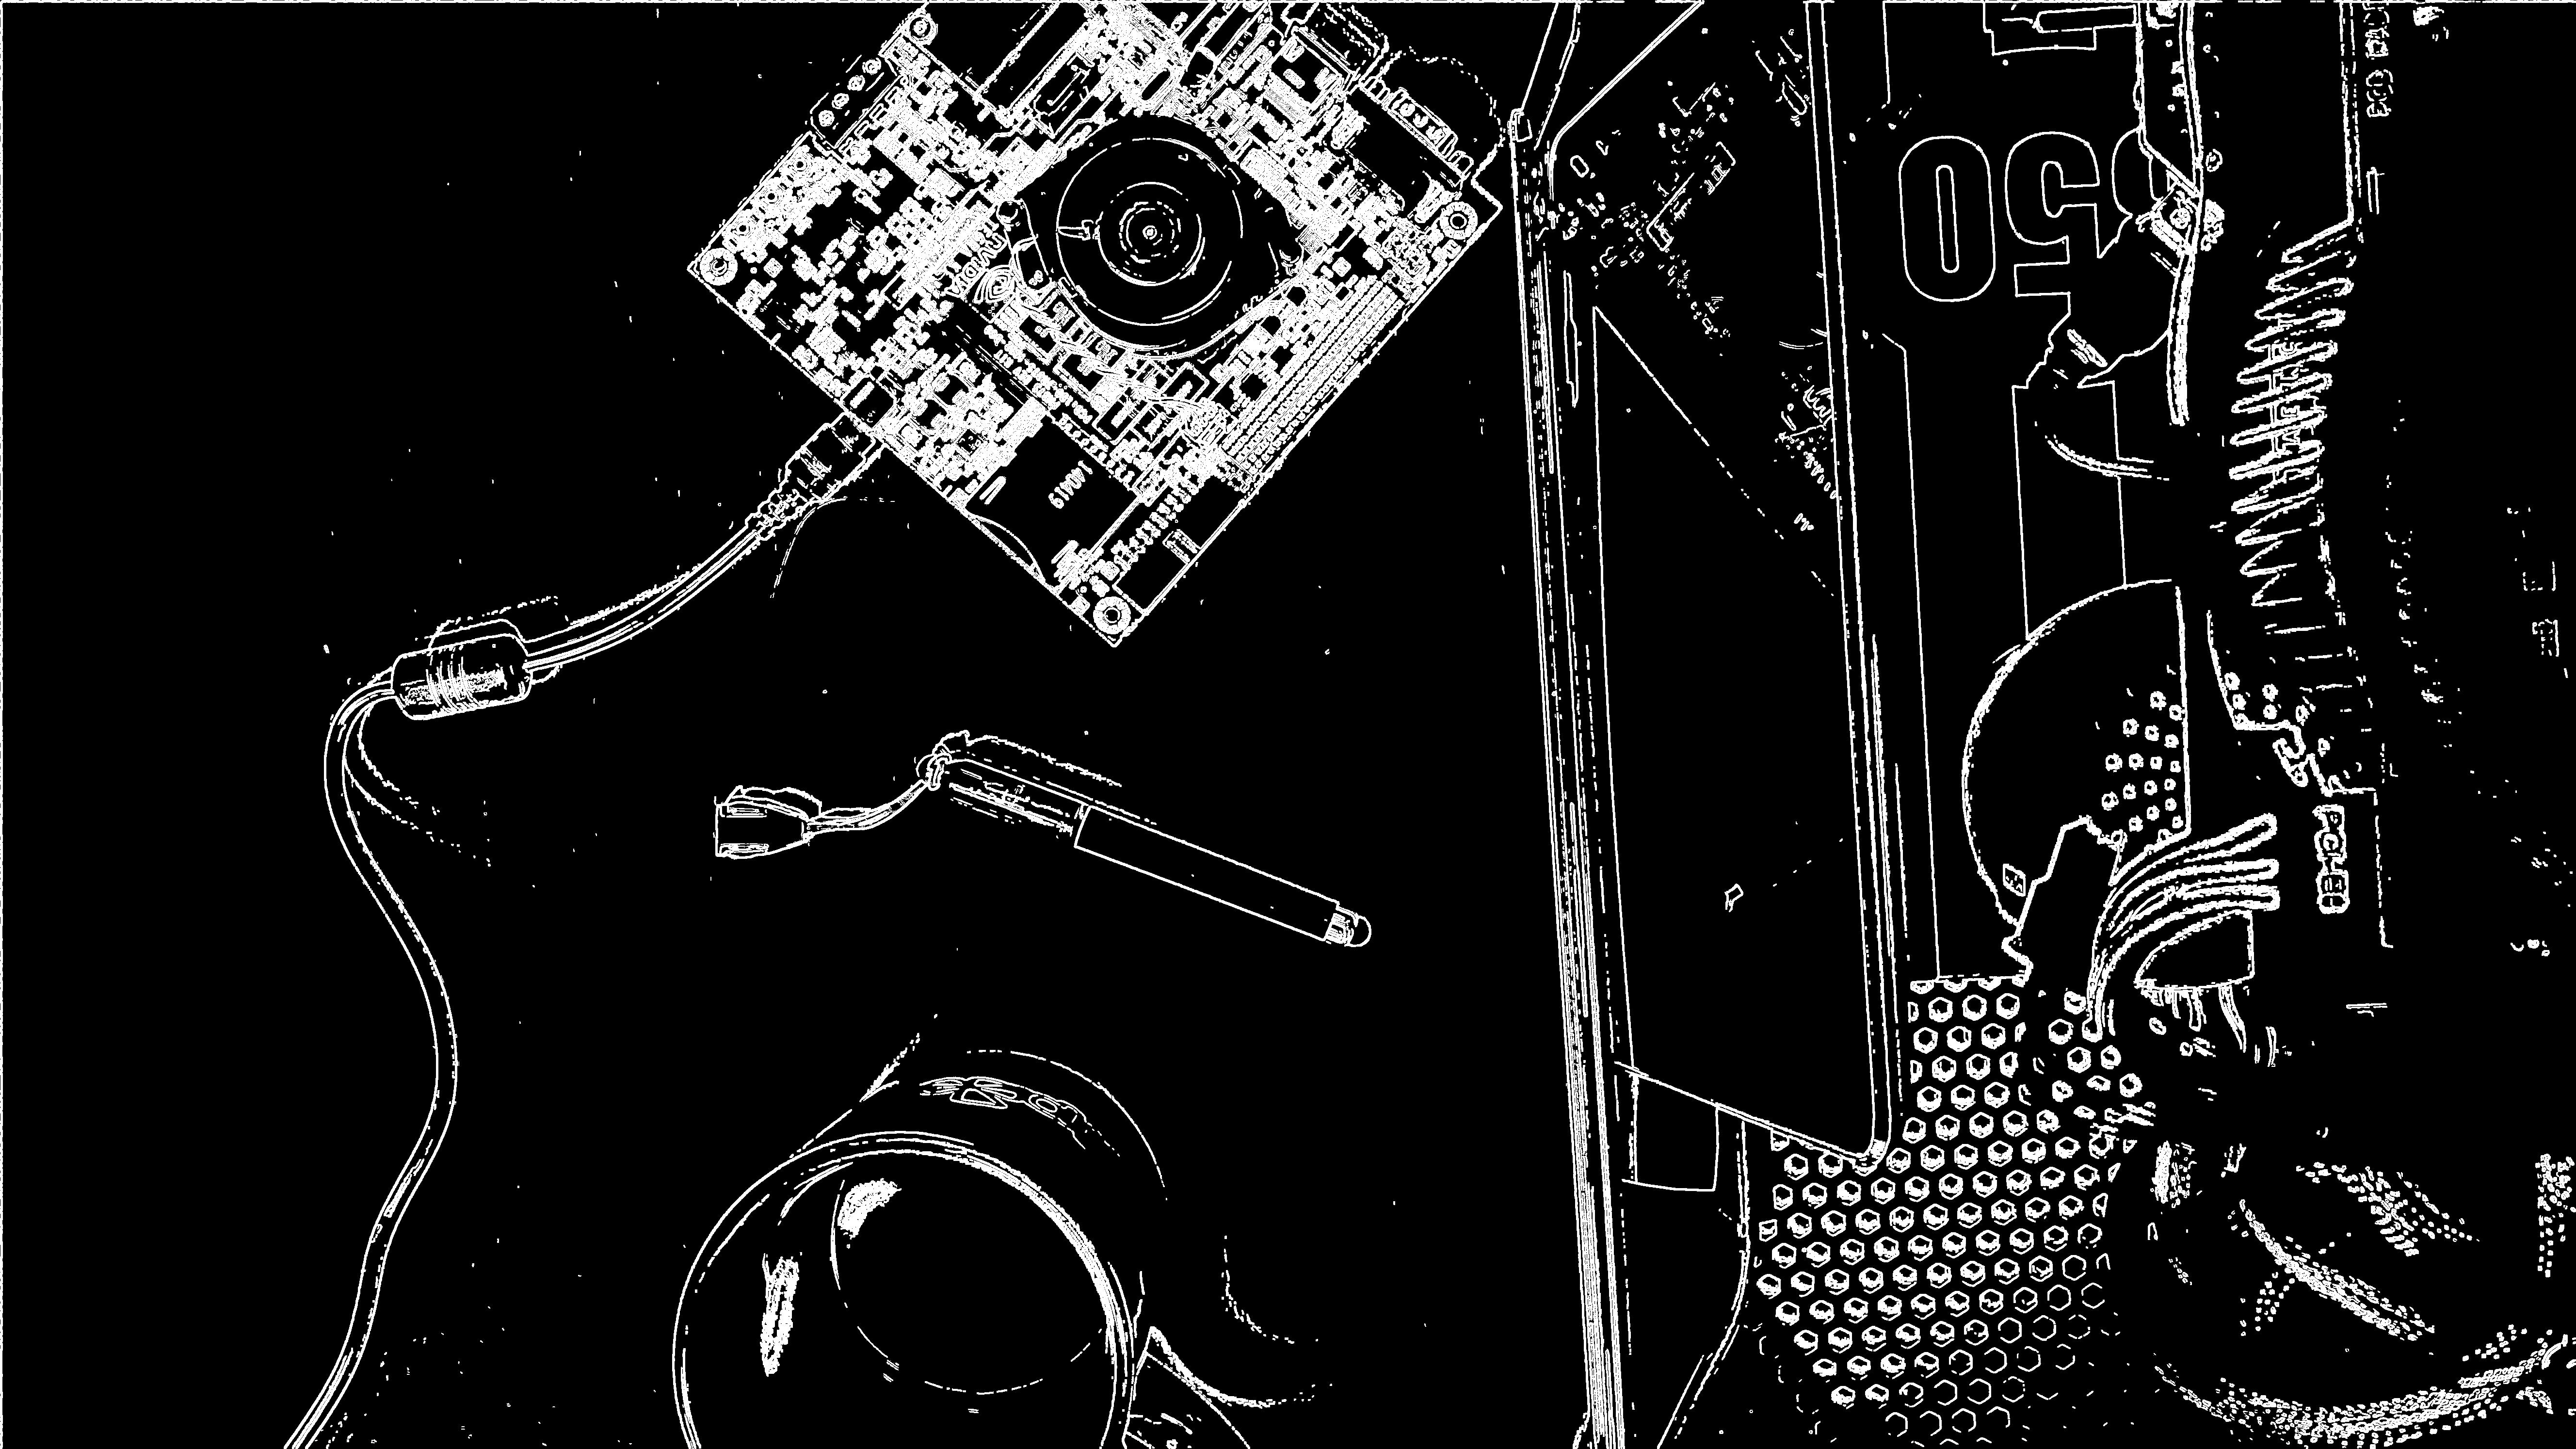
\includegraphics[width=0.45\textwidth]{desk_edges_1.jpg}
	\caption{Example of difference matrix computation: edges of the initial frame $\boldsymbol{E}_1$ computed with parameters $k = 5$, $\sigma = 5$, $t_l = 15$, $t_h = 25$}
    \label{desk-1-edges}
\end{figure}
\begin{figure}[H]
	\centering
	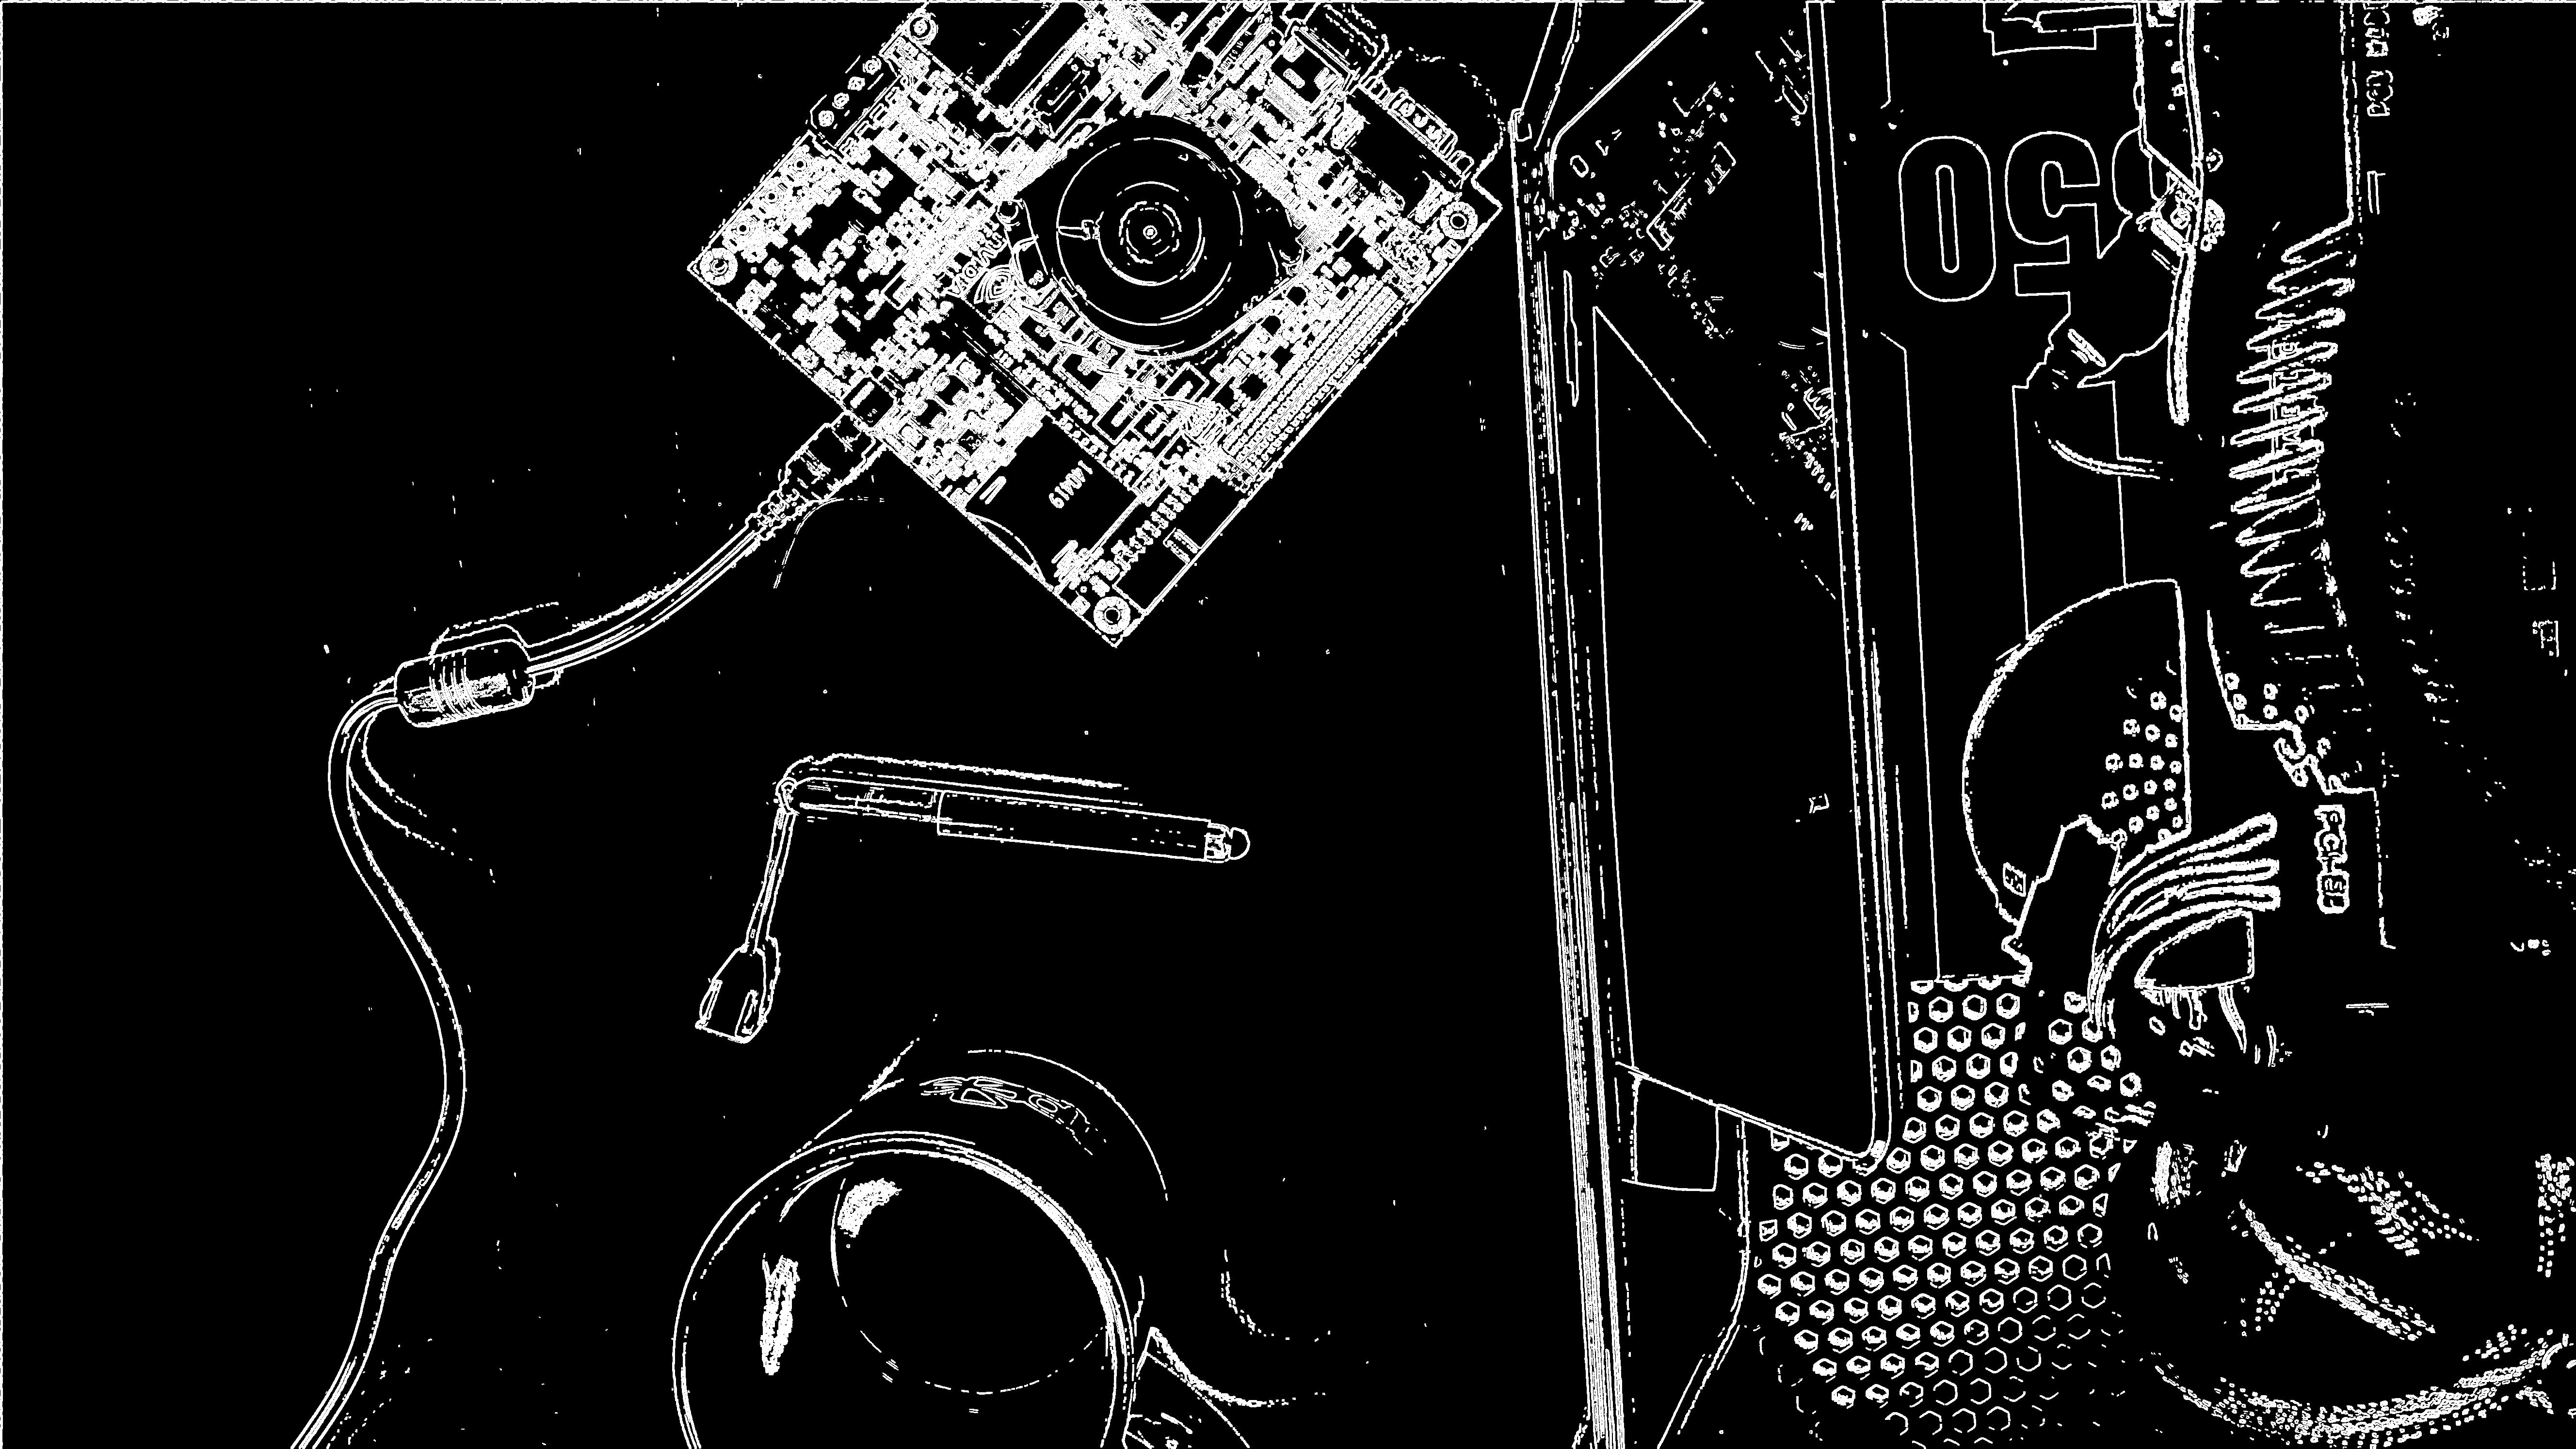
\includegraphics[width=0.45\textwidth]{desk_edges_2.jpg}
	\caption{Example of difference matrix computation: edges of the initial frame $\boldsymbol{E}_2$ computed with parameters $k = 5$, $\sigma = 5$, $t_l = 15$, $t_h = 25$}
    \label{desk-2-edges}
\end{figure}
\begin{figure}[H]
	\centering
	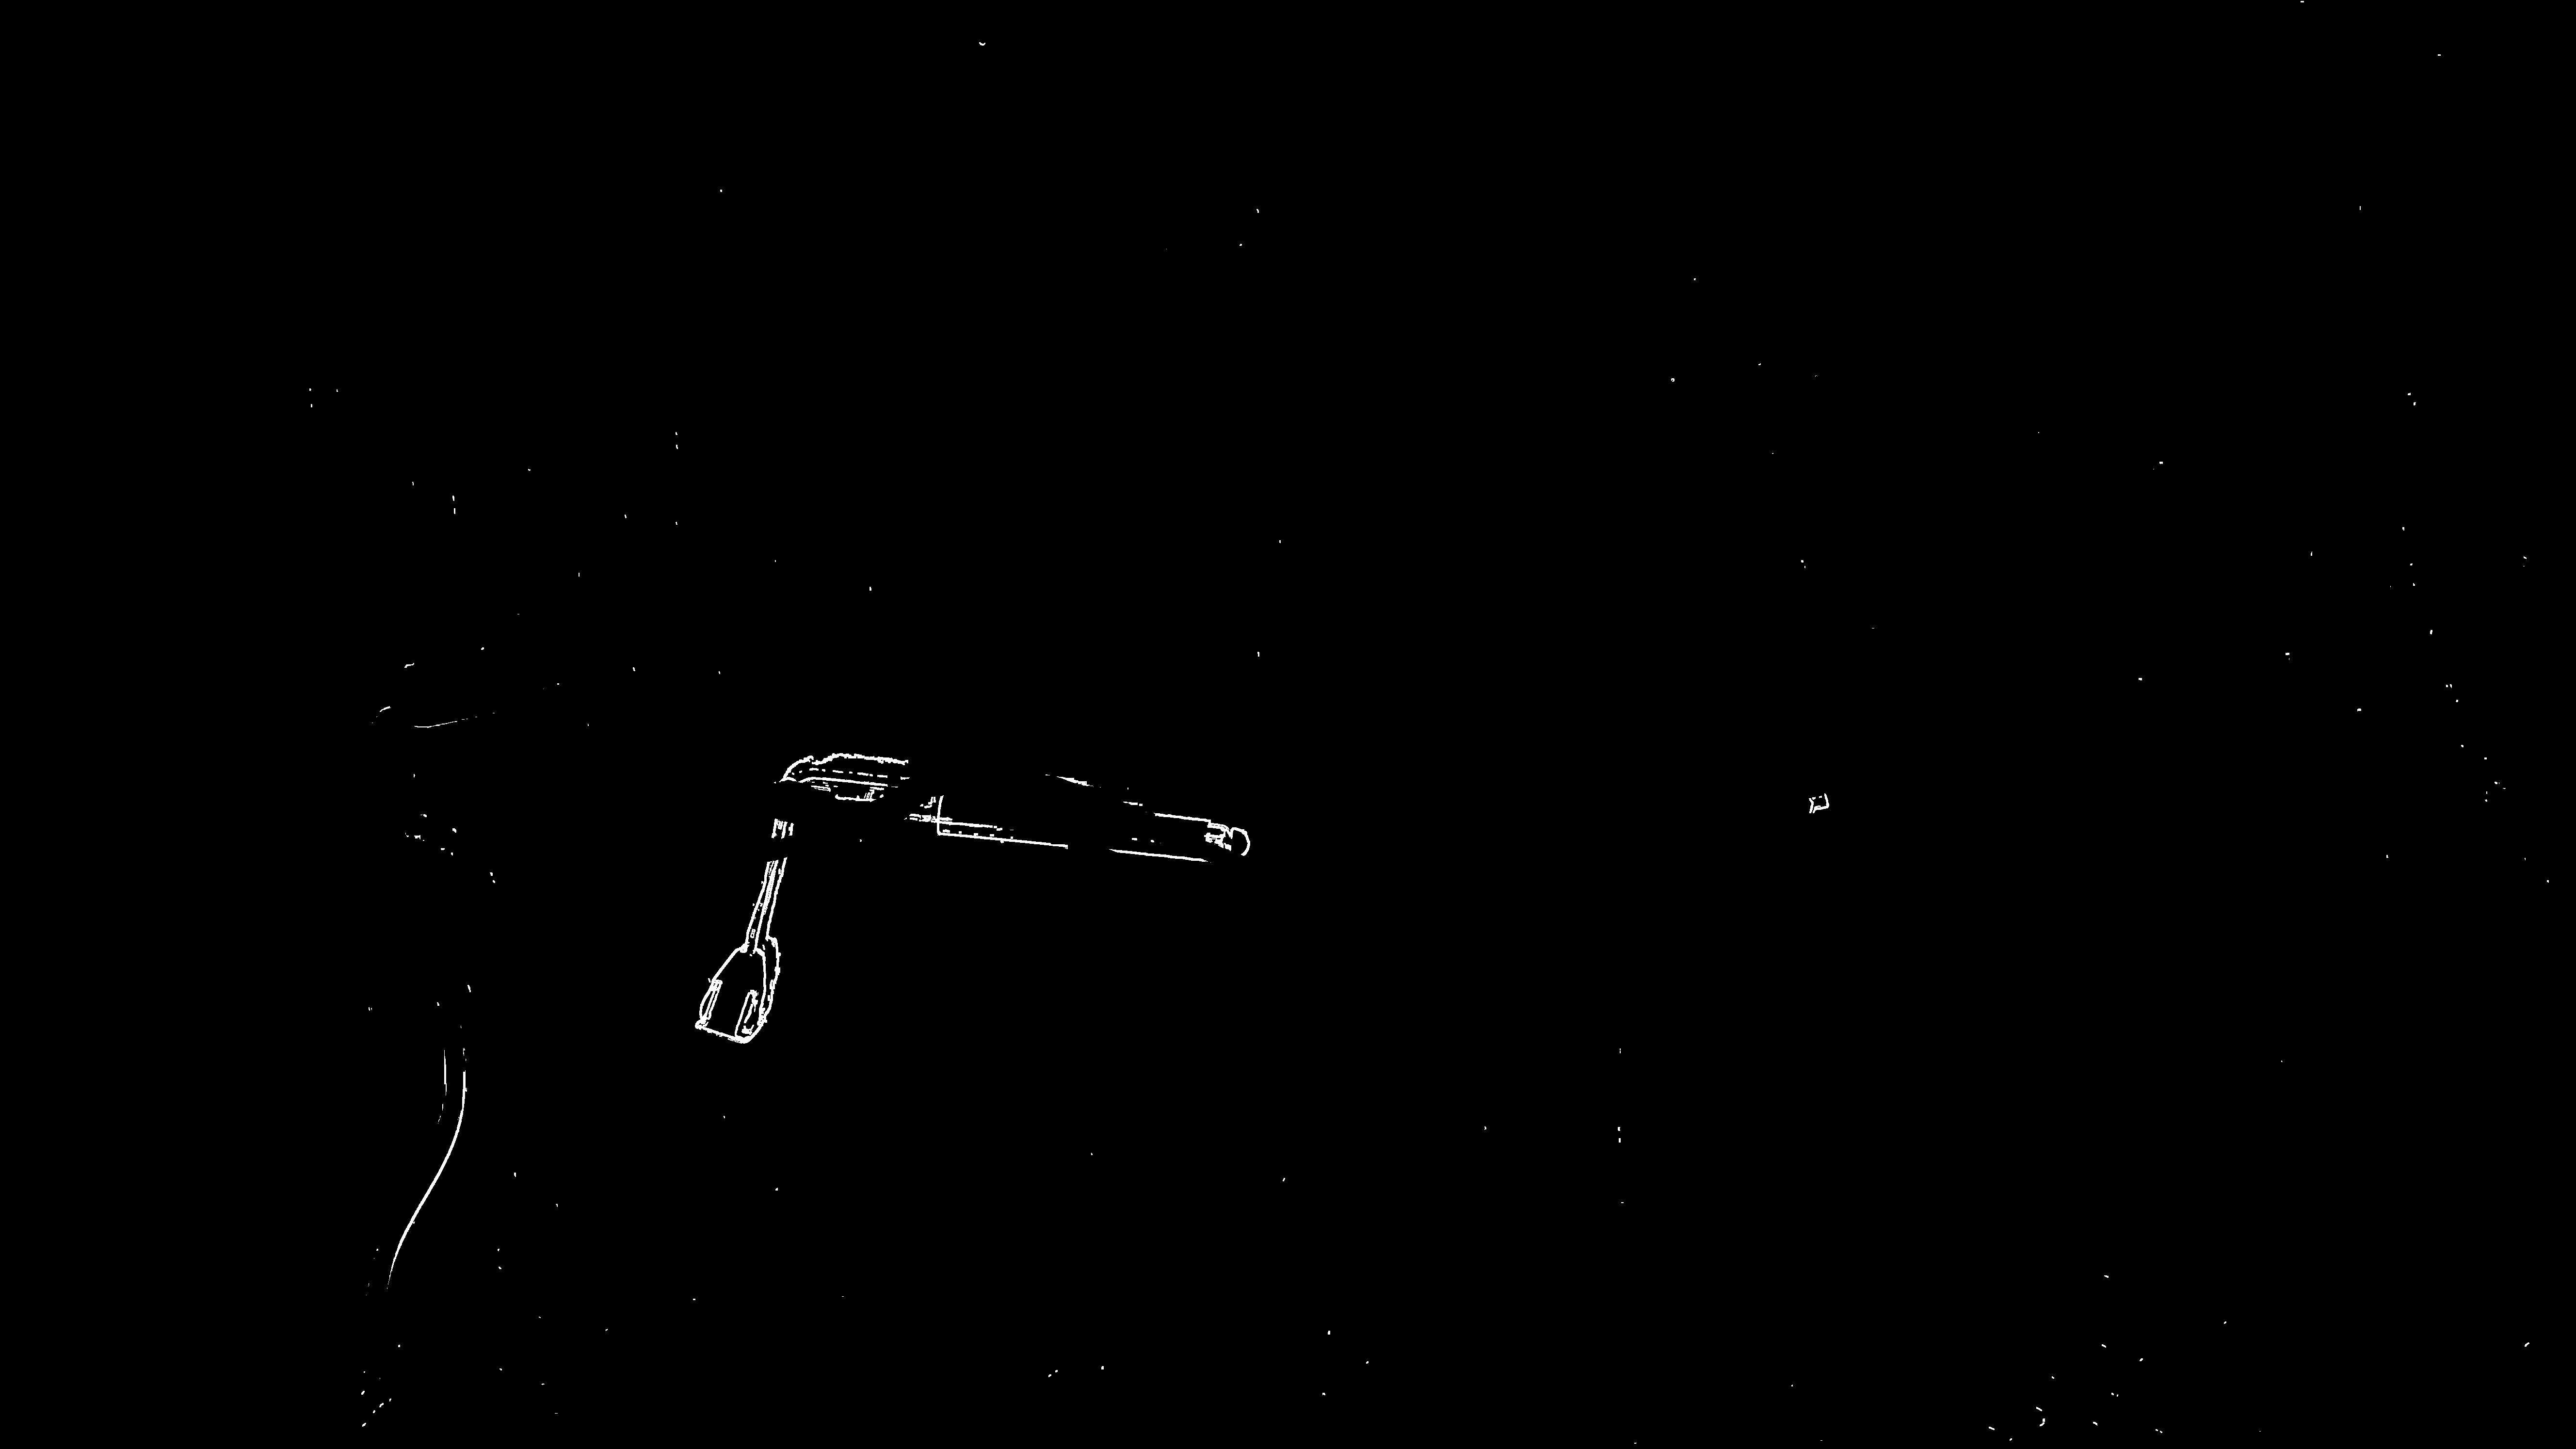
\includegraphics[width=0.45\textwidth]{desk_difference.jpg}
	\caption{Example of difference matrix computation: difference matrix $\boldsymbol{D}$ with parameter $\beta = 12$}
    \label{desk-difference}
\end{figure}
\begin{algorithm}[]
	\smaller
	\label{difference-matrix-algorithm}
	\caption{Determining the difference matrix between two frames, given their edge data: pseudocode for a serial, CPU implementation}
	
	\KwIn{Edge matrices $\boldsymbol{E}_1$ and $\boldsymbol{E}_2$, both of dimensions $M$ x $N$, and movement tolerance threshold $\beta$}
	\KwOut{Thresholded difference matrix $\boldsymbol{D}$; any entry $\boldsymbol{D}_{i, j}$ is $255$ if there is a difference, $0$ otherwise}
	
	\nl Initialize $\boldsymbol{D}_{i, j}$ to 0 $\forall i \in [0, M - 1], \forall j \in [0, N - 1]$\;
	\nl \ForEach {$i \in [0, M - 1]$} {
		\nl \ForEach {$j \in [0, N - 1]$} {
			\nl \If {$\boldsymbol{E}_{1_{i, j}} \neq \boldsymbol{E}_{2_{i, j}}$} {
				\nl $\boldsymbol{D}_{i, j} \gets 255$\;
				\ForEach {$i' \in [-\beta, \beta]$} {
					\ForEach {$j' \in [-\beta, \beta]$} {
						\nl \If{$(i + i', j + j')$ \textnormal{is within the bounds of} $E_1$ \textnormal{and} $\boldsymbol{E}_{1_{i + i', j + j'}} = \boldsymbol{E}_{2_{i + i', j + j'}}$} {
							\nl $\boldsymbol{D}_{i + i', j + j'} \gets 0$\;
						}
					}
				}
			}
		}
	}
	\nl \Return $\boldsymbol{D}$\;
	\
\end{algorithm}

\subsection{Motion Area Estimation via a Spatial Difference Density Map}
The difference matrix $\boldsymbol{D}$ determined with Algorithm \ref{difference-matrix-algorithm} is effectively a maximally precise estimate of motion area (e.g., to the resolution of a single pixel, since $\boldsymbol{D}$ is computed on a pixel-by-pixel basis). However, in practice, it is more useful to consider general regions of the image around which motion exists. For this reason, we build a density map of the matrix $\boldsymbol{D}$ using equal-sized rectangular sections of the input image that approximates the density of the difference per unit area (units pixels$^2$). Thus, the original $M \times N$ difference matrix $\boldsymbol{D}$ is reduced to a matrix $\boldsymbol{D}'$ of size $m \times n$ such that
$$M = k_1 m$$
$$N = k_2 n$$
where $k_1, k_2 \in \mathbb{Z}$. Intuitively, choosing a higher $k_1$ and $k_2$ will result in a higher resolution over which the density is evaluated. Selection of $k_1$ and $k_2$ should depend on how large of a region over which motion should be estimated. The upper limits of $k_1$ and $k_2$ are $M$ and $N$, respectively, at which point $\boldsymbol{D}'$ = $\boldsymbol{D}$. Each index $(m, n)$ in $\boldsymbol{D}'$ corresponds to the upper-left corner of a rectangular section of $\boldsymbol{A}$ whose width is $\frac{M}{m}$ and height is $\frac{N}{n}$.
\par Regions of motion are the rectangular sections whose density exceeds a user-defined threshold $\Gamma$, denoting the number of difference pixels over the total number of pixels considered in the rectangular section. For each such region $\boldsymbol{R}$ in $\boldsymbol{A}$ of size $\frac{M}{m}$ x $\frac{N}{n}$,
$$\textnormal{DifferenceDensity}(\boldsymbol{R}) = \frac{\textnormal{number of pixel differences in } \boldsymbol{R}}{\textnormal{number of pixels in } \boldsymbol{R}}$$
\[
\boldsymbol{D}' =
\begin{cases}
1 & \textnormal{DifferenceDensity}(\boldsymbol{R}) > \Gamma\\
0 & \textnormal{otherwise}
\end{cases}
\]
\begin{figure}[]
	\centering
	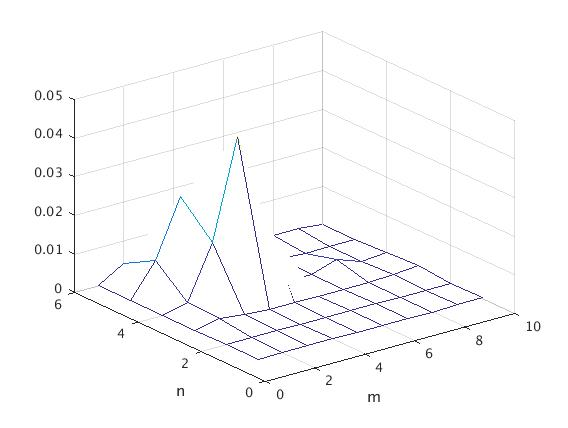
\includegraphics[width=0.45\textwidth]{desk_difference_density.jpg}
	\caption{Spatial difference density matrix $\boldsymbol{D}'$ (visualized in three dimensions) of Figure \ref{desk-difference}, as determined by Algorithm \ref{difference-density-matrix-algorithm} with parameters $m = 10$, $n = 6$, and $\Gamma = 0.01$}
    \label{desk-difference-density}
\end{figure}
\begin{figure}[]
	\centering
	
\includegraphics[width=0.45\textwidth]{desk_motion_area.jpg}
	\caption{Final estimate of motion area of Figures \ref{desk-1-original} and \ref{desk-2-original} based on the density map of Figure \ref{desk-difference-density}}
    \label{desk-motion-area}
\end{figure}
\begin{algorithm}[]
	\smaller
	\label{difference-density-matrix-algorithm}
	\caption{Estimating regions of motion in an image with a difference density matrix: pseudocode for a serial, CPU implementation}
	
	\KwIn{Thresholded difference matrix $\boldsymbol{D}$, motion threshold $\Gamma$, width of the original image $M$, height of the original image $N$, number of horizontal divisions $m$, and number of vertical divisions $n$}
	\KwOut{The difference density matrix $\boldsymbol{D}'$ of dimensions $m$ x $n$ whose value is 1 if there is motion in that region, and 0 otherwise}
	
	\nl Initialize $\boldsymbol{D}'$ to 0 $\forall i \in [0, m - 1], \forall j \in [0, n - 1]$\;
	\nl \ForEach {$i \in [0, m - 1]$} {
		\nl \ForEach {$j \in [0, n - 1]$} {
			\nl $x \gets 0$\tcp*{Number of differences in this region}
			\nl \ForEach{$i' \in [0, \frac{M}{m}]$} {
				\nl \ForEach{$j' \in [0, \frac{N}{n}]$} {
					\nl \If {$\boldsymbol{D}_{\frac{Mi}{m} + i', \frac{Nj}{n} + j'} \neq 0$} {
						\nl $x \gets x + 1$\;
					}
				}
			}
			\nl \If{$\frac{mn}{MN}x > \Gamma$} {
				\nl $\boldsymbol{D}'_{i, j} \gets 1$\;
			}
		}
	}
	\nl \Return $\boldsymbol{D}'$\;
	\
\end{algorithm}


\subsection{GPU Parallelization and CUDA Implementation}
Our CUDA implementation of our motion detection algorithm is similar to that for our implementation of separable convolution and edge detection. Using the same 16 threads per block, we divide the input image into the appropriate number of blocks such that the thresholded difference computation at each index $(i, j)$ of Algorithm \ref{difference-matrix-algorithm} has its own thread. Thus, each element of $\boldsymbol{D}$ is calculated in parallel.
\begin{lstlisting}[
	caption=GPU computation of thresholded difference matrix,
	label=difference-filter-implementation,
	language=C
]
__global__ void difference_filter(
	int *dev_out,
	int *edges_1,
	int *edges_2,
	int width,
	int height,
	int threshold
) {
	const int r = blockIdx.y * blockDim.y + threadIdx.y;
	const int c = blockIdx.x * blockDim.x + threadIdx.x;
	const int i = r * width + c;

    // Set it to 0 initially
    dev_out[i] = 0;
    int crop_size = 7;
    if (r > crop_size && c > crop_size && r < height - crop_size && c < width - crop_size && edges_1[i] != edges_2[i]) {
        // Set to 255 if there is a pixel mismatch
        dev_out[i] = 255;
        for (int x_apron = -threshold; x_apron <= threshold; x_apron++) {
            for (int y_apron = -threshold; y_apron <= threshold; y_apron++) {
                // Ensure the requested index is within bounds of image
                if (c + x_apron > 0 && r + y_apron > 0 && c + x_apron < width && r + y_apron < height) {
                    // Check if there is a matching pixel in the apron, within the threshold
                    if (edges_1[(r + y_apron) * width + c + x_apron] == edges_2[i]) {
                        // Set it back to 0 if a corresponding pixel exists within the vicinity of the match
                        dev_out[i] = 0;
                    }
                }
            }
        }
    }
}
\end{lstlisting}
The construction of the difference density matrix as in Algorithm \ref{difference-density-matrix-algorithm} is parallelized by considering the value of the thresholded difference matrix $\boldsymbol{D}'$ at each index $(r, c)$, mapping that index to the appropriate index in the difference density matrix $(i, j)$ where $i < m \wedge j < n$, then adding to the value of the array at $(i, j)$ at each encounter of a difference pixel in $\boldsymbol{D}'$. Our CUDA implementation therefore relies on the fact that the density array is initialized to 0 before the kernel is launched; this is accomplished in practice with a \texttt{calloc} operation on the host, followed by copying that array to GPU memory.
\begin{lstlisting}[
	caption=GPU computation of the difference density matrix,
	label=difference-density-implementation,
	language=C
]
__global__ void spatial_difference_density_map(
	double *density_map,
	int *difference,
	int width,
	int height,
	int horizontal_divisions,
	int vertical_divisions
) {
	int r = blockIdx.y * blockDim.y + threadIdx.y;
	int c = blockIdx.x * blockDim.x + threadIdx.x;
	int i = r * width + c;
	
	int horizontal_block_size = width/horizontal_divisions;
	int vertical_block_size = height/vertical_divisions;
	int block_size = horizontal_block_size * vertical_block_size;
	
	const int scaling_factor = 1000;
	if (difference[i] != 0) {
		int i = (int)(vertical_divisions * r/(double)height);
		int j = (int)(horizontal_divisions * c/(double)width);
		density_map[i * horizontal_divisions + j] += scaling_factor/(double)block_size;
	}
}
\end{lstlisting}
The generation of the motion area estimation image is relatively straightforward: we map the index $(i, j)$ of $\boldsymbol{D}'$ back to an index $(r, c)$ where $r < M \wedge c < N$, and set the value at that index high or low accordingly.
\begin{lstlisting}[
	caption=GPU generation of the motion area estimation image,
	label=motion-area-estimation-implementation,
	language=C
]
__global__ void motion_area_estimate(
	int *motion_area,
	double *density_map,
	int width,
	int height,
	int horizontal_divisions,
	int vertical_divisions,
	double threshold
) {
	int r = blockIdx.y * blockDim.y + threadIdx.y;
	int c = blockIdx.x * blockDim.x + threadIdx.x;
	int i = r * width + c;
	
	int density_map_index = (int)(vertical_divisions*r/(double)height) * horizontal_divisions + (int)(horizontal_divisions*c/(double)width);

	if (density_map[density_map_index] >= threshold) {
		motion_area[i] = 255;
	} else {
		motion_area[i] = 0;
	}
}
\end{lstlisting}

\subsection{High-Level Python Implementation}
The Python implementation of Algorithm \ref{difference-density-matrix-algorithm} is very straightforward and looks almost exactly like the pseudo-code, making it easy to implement even for those with minimal programming experience.
\begin{lstlisting}[
	caption=Python implementation of the motion area estimation image,
	label=python-motion-area-estimattion-implementation,
	language=Python
]
import numpy as np

def detect_motion(e1, e2):
    height, width, depth = np.shape(e1)
    d = difference(e1, e2)
    d_prime = np.zeros((M, N), np.uint8)
    for i in range(M):
        for j in range(N):
            x = 0
            for i_prime in range(height/M):
                for j_prime in range(width/N):
                    if d[i*height/M+i_prime, j*width/N+j_prime] != 0:
                        x += 1
            if M*N*x/(height*width*1.0) > T:
                d_prime[i, j] = 255
    return d_prime
\end{lstlisting}


\section{Facial Recognition Algorithm}
\label{facial-recognition-section}
Our facial recognition implementation is based off of the HAAR features-based cascade classifiers method proposed by Viola-Jones in 2001. It's split into two phases: training and detection. The algorithm is as follows:
\begin{enumerate}
	\item Extract HAAR features of a face from a set of positive and negative training images. 
	\item Use adaptive boosting machine learning to train a multi-stage, or cascade, classifier against positive and negative HAAR features. 
	\item Apply a final cascade classifier to a loaded image or real time video frame. 
\end{enumerate}
Due to the resource capacity necessary to train a full facial recognition classifier, we used a pre-trained frontal face cascade classifier and used OpenCV's object detection library, which encapsulates the algorithm above, and whose theory detailed in the following sections.

\subsection{HAAR Feature Extraction}
In mathematics analysis, Haar wavelets are a sequence of rescaled, square-like functions. In image processing, Haar features are so named for their resemblance to Haar wavelets. Haar features are regularities identified in all human faces, by comparing light and dark gradients across the face. These are split into edge (two-rectangle) features, line (three-rectangle) features, and diagonal (four-rectangle) features.
\begin{figure}[h]
	\centering
	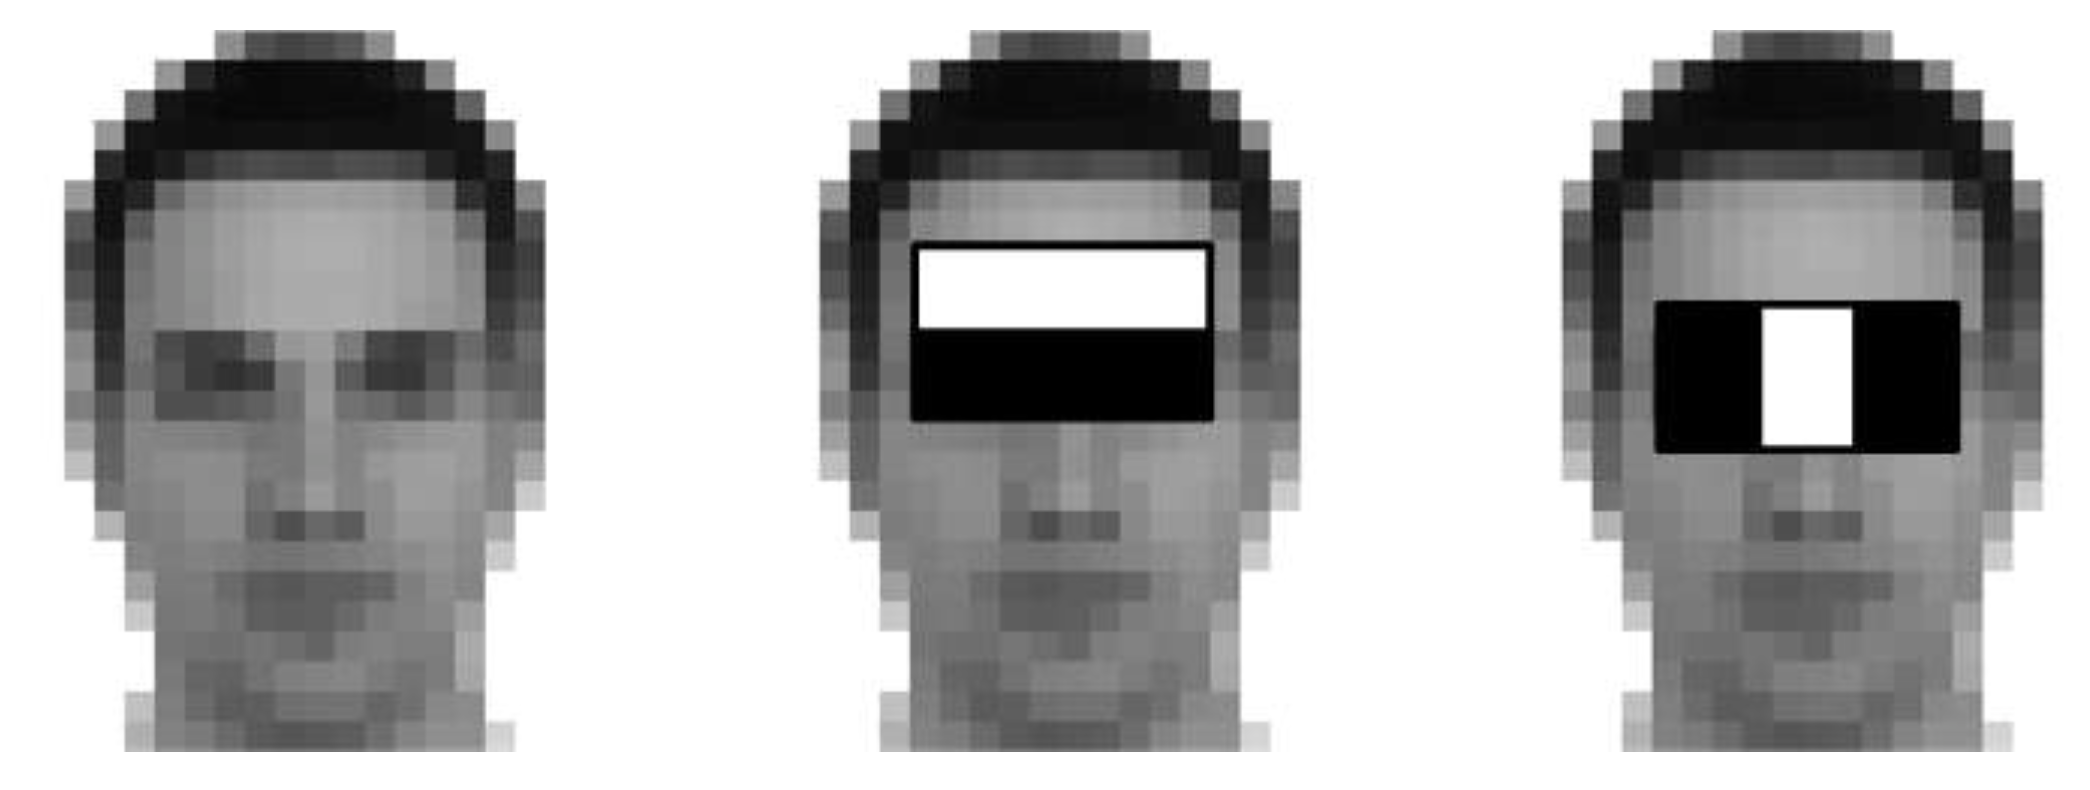
\includegraphics[width=0.45\textwidth]{haar_features.png}
	\caption{Example application of HAAR features on a face}
    \label{haar-features-face-example}
\end{figure}
\par Each feature is obtained by comparing the pixel intensity in the white boxes against the pixel intensity in the dark boxes for a wide sample of sub-windows across the entire image. A 24x24 pixel image window can produce over 160,000 features that need to be classified, in some sense, “oversampling” the face.
\par The rectangle features can be computed by splitting the image into sub-windows called integral images. An integral image at a point $i'(x, y)$ is the sum of all pixels to the top and to the left of that point.
\[
i'(x, y) = \sum_{m \leq x, n \leq y}{i(m, n)}
\]
\begin{figure}[h]
	\centering
	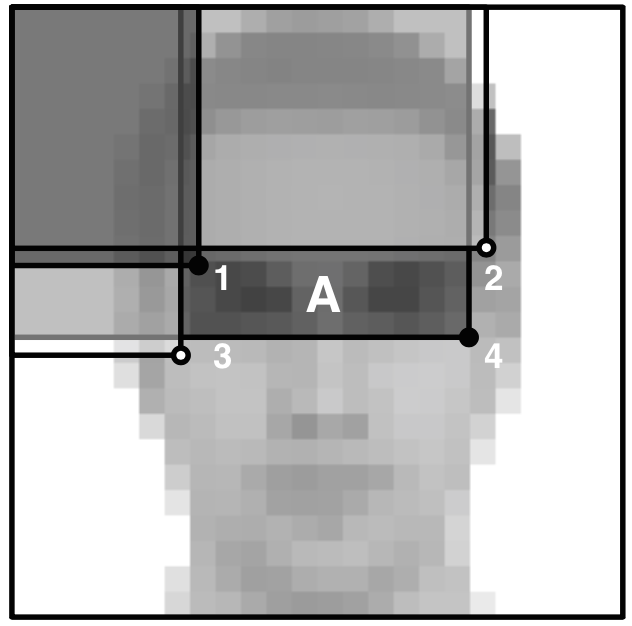
\includegraphics[width=0.45\textwidth]{integral_image.png}
	\caption{Integral image on a face}
    \label{integral-image-face}
\end{figure}
Since an integral image includes all previously-computed integral images contained in its window, in the image of Figure \ref{integral-image-face}, the region A can be computed as
\[
A = i'(4) + i'(1) - i'(2) - i'(3)
\]
Any such rectangular sum can be computed using four array references.

\subsection{Cascade Classifier Training}
It's far too resource intensive to evaluate over 160,000 images for each 24x24 pixel window. However, we can take advantage of the fact that only a very small fraction of extracted sub-windows in an uncropped image will correspond to accurate facial features. To do so, we use a cascaded variation of the Adaptive Boosting (or AdaBoost) machine learning algorithm. AdaBoost aims to determine the optimal binary threshold of HAAR features which best separate negative and positive samples.
\begin{algorithm}[]
	\smaller
	\label{adaboost-classifier-algorithm}
	\caption{AdaBoost classifier training}
	
	\KwIn{Set of training images $I$, where each image $i \in I$ is a two-dimensional matrix representing the image, and is labeled as either a positive or negative sample image; $m$, the number of positive samples; $l$, the number of negative samples; $F$, the set of features extracted from images in $I$; $\theta_f, \forall f \in F$, denoting a threshold for weakly classifying a feature match}
	\KwOut{Strong classifier function $h(x)$ whose value is $1$ if the image $x$ contains a face, and $0$ otherwise}
	
	\nl Initialize $w$ to a mapping from images to image weights\;
	\nl Initialize $t$ to a mapping from images to the constant $1$ or $0$\;
	\nl \ForEach {$i \in I$} {
		\nl \If {$i$ \textnormal{is a positive training sample}} {
			\nl $t_i \gets 1$\;
			\nl $w_i \gets \frac{1}{2m}$\;
		}
		\nl \Else {
			\nl $t_i \gets 0$\;
			\nl $w_i \gets \frac{1}{2l}$\;
		}
	}
	\nl \ForEach {$f \in F$} {
	\nl $g_f \gets \textnormal{ trained weak classifier  } \begin{cases}1 & \textnormal{value of } f < \theta_f \\ 0 & \textnormal{else}\end{cases}$\;
		\nl \ForEach {$i \in I$} {
			\nl $w' \gets w \textnormal{ normalized such that } \sum_{k \in I} w_k = 1$\;
			\nl $\varepsilon_f \gets \textnormal{the minimum value of the error } \sum_{k \in I} w'_k |g_f(i) - t_i|$\;
			\nl $\beta_f \gets \textnormal{weight inversely proportional to } \varepsilon_f$\;
			\nl $w_i \gets \beta_f w'_i$\;
		}
	}
	\nl $h(x) \gets \begin{cases}1 & \sum_{f \in F} g_f(x) \log{\frac{1}{\beta_f}} \geq \frac{1}{2} \sum_{f \in F} \log{\frac{1}{\beta_f}} \\ 0 & \textnormal{else}\end{cases}$\;
	\nl \Return $h(x)$\;
	\
\end{algorithm}
\par From one pass at the AdaBoost algorithm, it is clear that running hundreds of thousands of features on millions of samples will be too computationally intensive. However, most features in a general, uncropped image do not correspond to a face. This allows us to set up a cascaded variant of the AdaBoost algorithm.
\par In cascading, all the features are grouped into several stages, where each stage checks for a certain amount of features. It's set up such that the most common facial features are grouped into the earliest cascade stages. This allows us to discard most non-facial regions early on and only spend successive computations on potentially positive regions. If a region fails during a stage, it is discarded, the cascade training stops, and then resets at the next potentially positive region. This vastly improves resource and time efficiency of classifier training.
\begin{figure}[h]
	\centering
	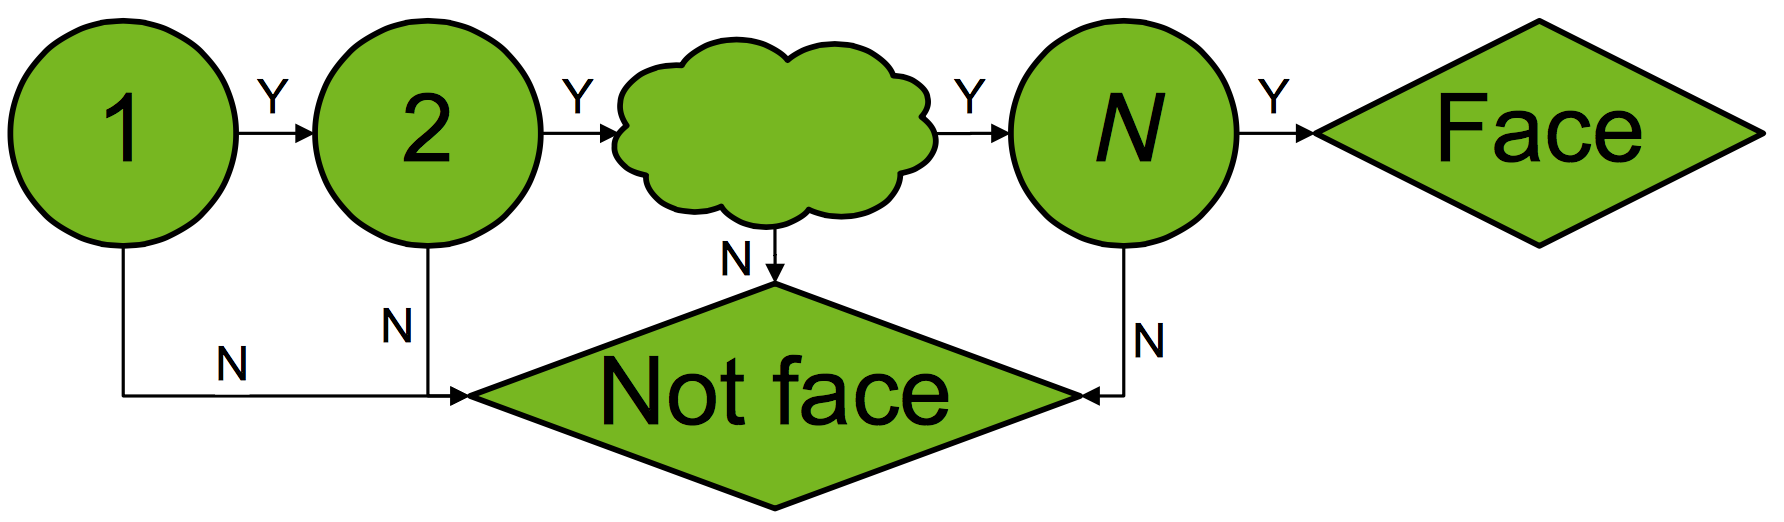
\includegraphics[width=0.45\textwidth]{cascade_framework.png}
	\caption{Cascade training framework}
    \label{cascade-framework}
\end{figure}

\subsection{Application of Classsifier to Facial Recognition}
The final output of the cascade classifier training is a classifier XML file that contains the results of the training. OpenCV then provides an easy module to apply that XML file to real time face detection. We just need to import the file, pre-process our images (or frames from real-time video stream), and then run the OpenCV object detection functions.
\par We load the trained classifier, load our image, and then the object detect functions returns the position of any found faces as a Rectangle with identifiers (x, y, width, height). With the returned positions, we can draw a basic rectangle of the detected facial regions or even perhaps take it a step further and apply Daft Punk masks to any detected faces.
\begin{figure}[H]
	\centering
	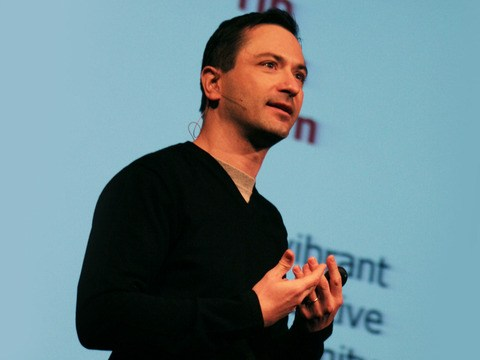
\includegraphics[width=0.45\textwidth]{richb.jpg}
	\caption{Sample input image to the classification}
    \label{richb}
\end{figure}
\begin{figure}[H]
	\centering
	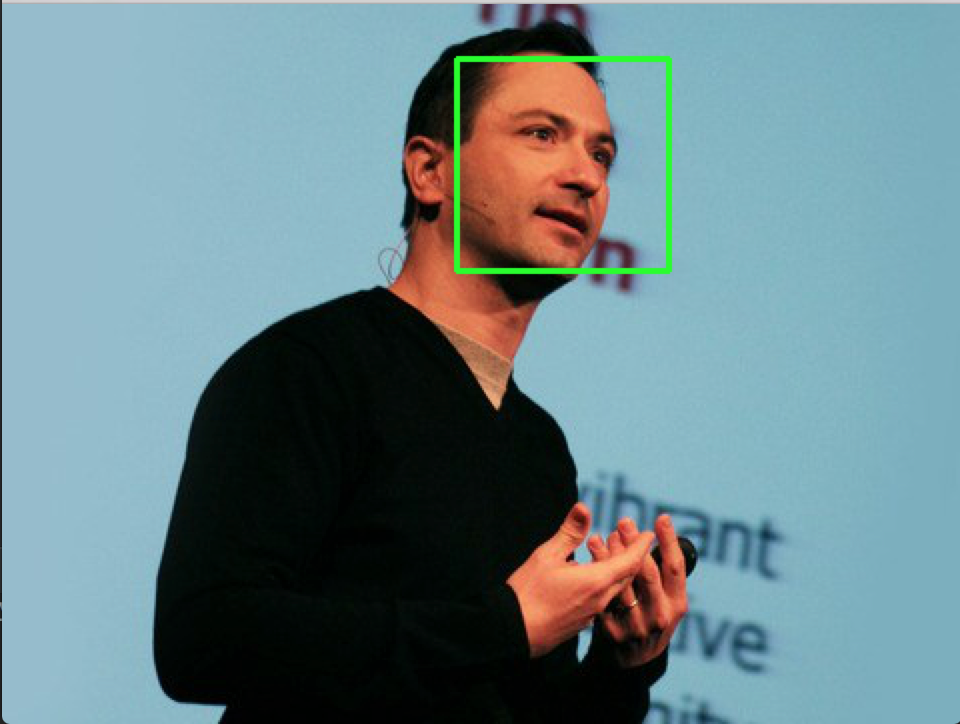
\includegraphics[width=0.45\textwidth]{richb_face_detected.png}
	\caption{Detected faces from the image of Figure \ref{richb} using the trained Frontal Face HAAR classifier}
    \label{richb-face-detected}
\end{figure}
\begin{figure}[h]
	\centering
	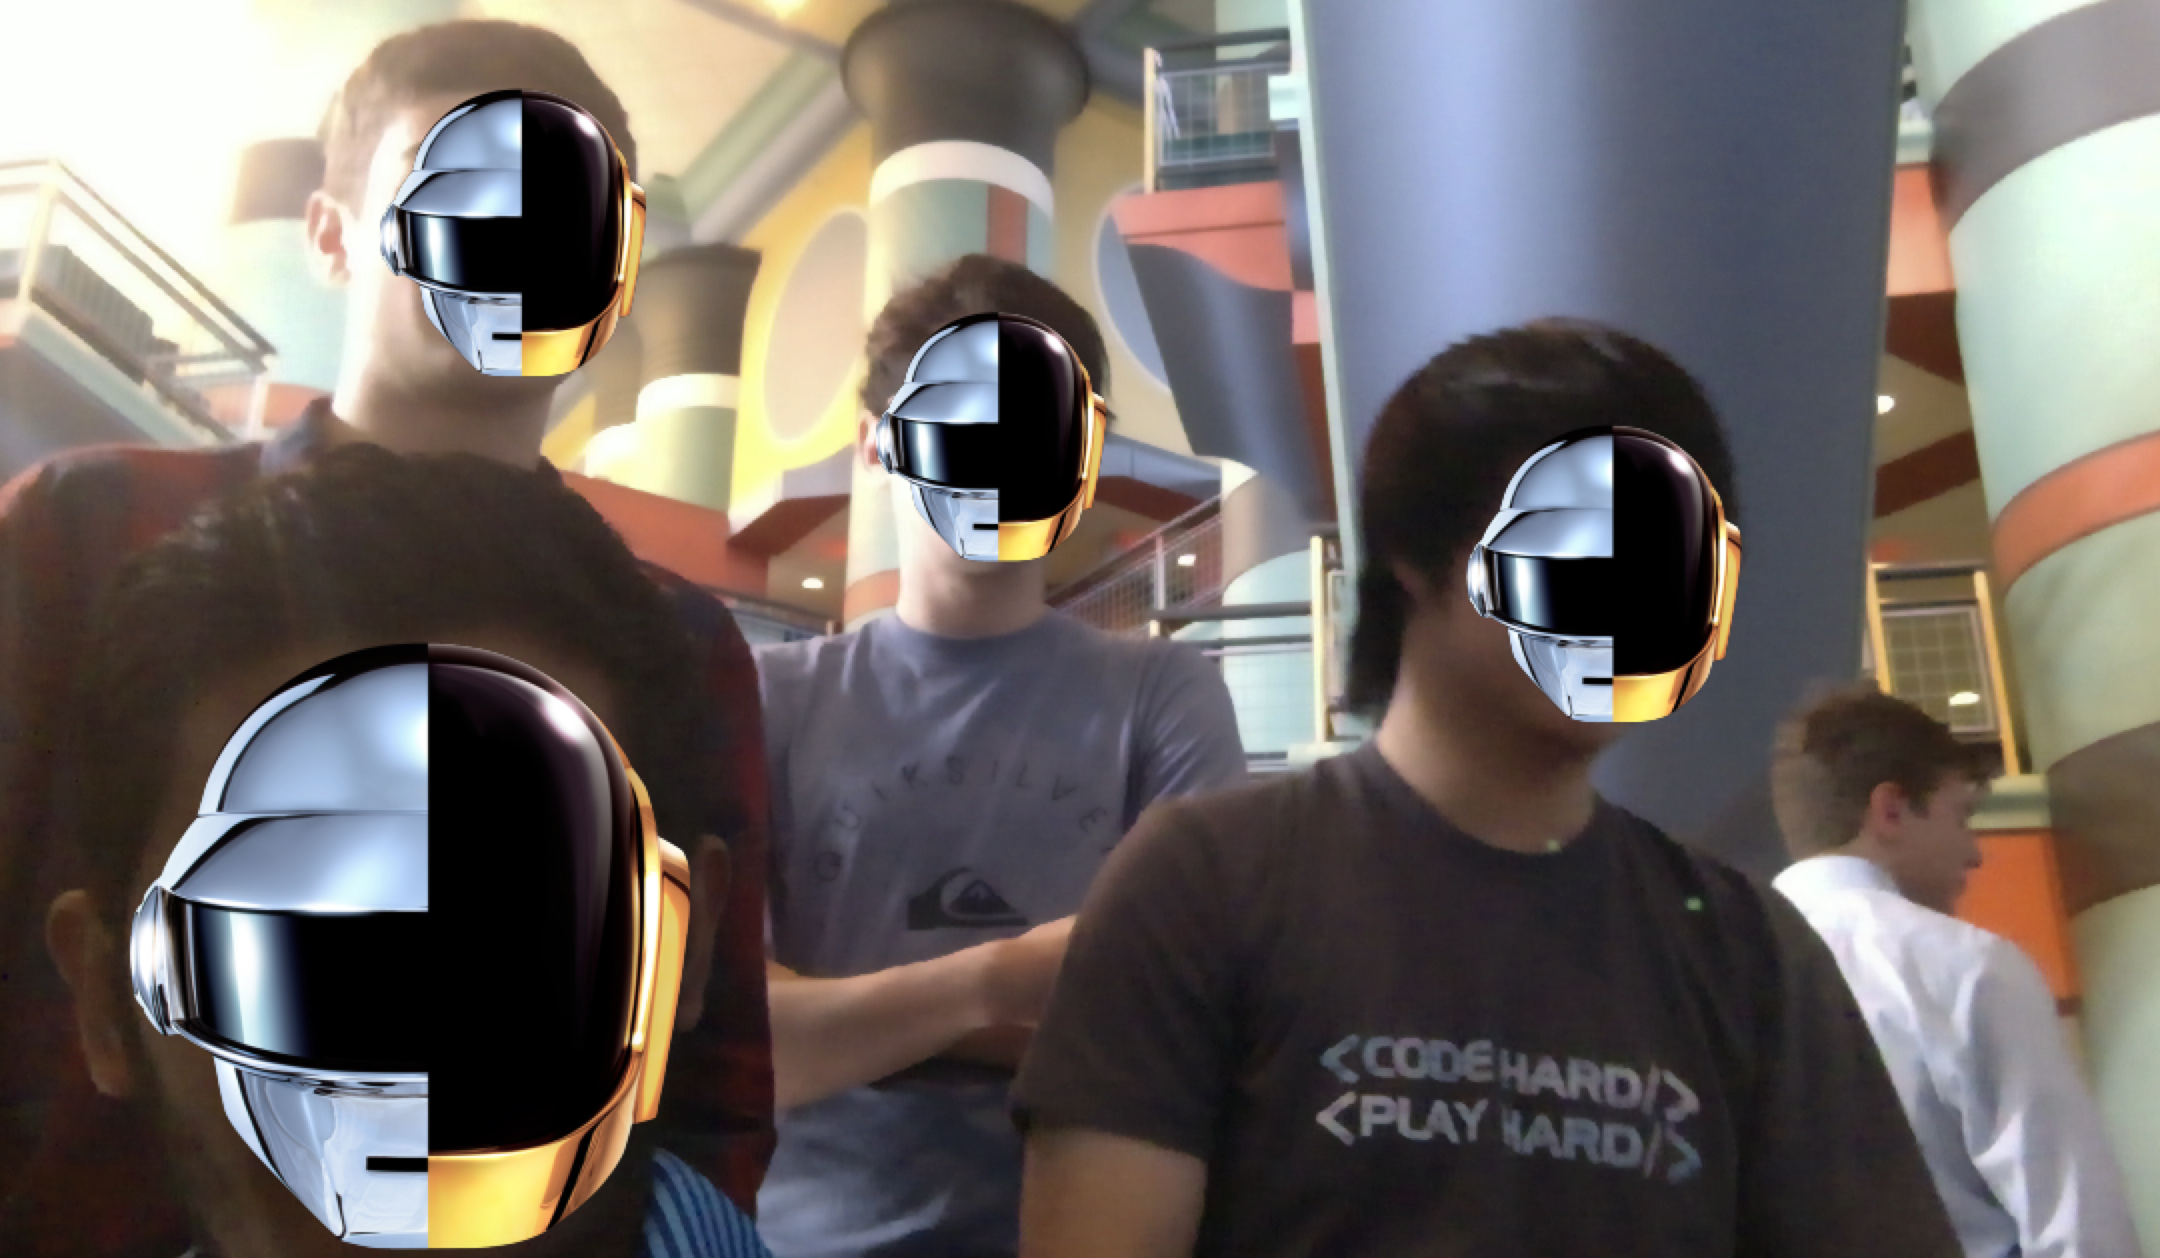
\includegraphics[width=0.45\textwidth]{daft_punk_masks.png}
	\caption{Sample application of facial recognition: scale-invariant Daft Punk masks applied to detected facial regions in real-time}
    \label{daft-punk-masks}
\end{figure}


\subsection{High-Level Python Implementation}
We again provide sample Python code to demonstrate how the facial recognition algorithm would be implemented on a high level, with the details of implementation abstracted out. The Python OpenCV library exposes an API for facial recognition via a cascade classifier, as shown in Listing \ref{python-facial-recognition-implementation}.
\begin{lstlisting}[
	caption=Python implementation of facial recognition with OpenCV,
	label=python-facial-recognition-implementation,
	language=Python
]
import cv2

IMAGE = 'richb.jpg'
CASCADE_DATA = 'haarcascade_frontalface_default.xml'

face_cascade = cv2.CascadeClassifier(CASCADE_DATA)
faces = face_cascade.detectMultiScale(
	cv2.imread(IMAGE, cv2.IMREAD_GRAYSCALE),
	scaleFactor=1.1,
	minNeighbors=5,
	minSize=(30, 30),
	flags=cv2.CASCADE_SCALE_IMAGE,
)
# faces now contains tuples indicating the location and size of each detected face in the image
\end{lstlisting}


\subsection{GPU Parallelization and CUDA Implementation}
The CUDA implementation in OpenCV's object detection framework takes advantage of the inherent parallelization available in pre-processing the images and traversing all of the image sub-windows.
\par Unlike previously with the edge detection and motion detection, where there is no singularly accepted CUDA implementation of the aforementioned algorithms, with facial recognition, OpenCV's library has been heavily optimized over the years to provide that functionality.
\par It would an interesting case study then to abstract the functionalities of their object detection libraries, and compare the speedups attained from using a heavily optimized 3rd party library against the speedups which we obtained from programs written by us from scratch.
\par OpenCV's CUDA implementation is similar to its serial CPU implementation, except that the cascade classifier is loaded in a CUDA optimized format, and the images are loaded and processed in CUDA-optimized matrices formats created by OpenCV. 


\section{GPU Speedup Results}
\label{results}
Our code for separable convolution, computation of the image's gradient magnitude and angle, non-maximum suppression and selective thresholding, and computation of the thresholded difference and spatial difference density matrices has both serial CPU and parallel CUDA implementations. Both the CPU and GPU implementations of the entire facial recognition algorithm are encapsulated in an OpenCV library internally implemented with CUDA. Here, we present speedup results for each of these procedures on various image sizes obtained on a system with the following hardware:
\begin{itemize}
	\item Intel Core i5 4200U @ 2.6 GHz (2C, 4T)
	\item 8 GB of DDR3 memory @ 1600 MHz
	\item NVIDIA GeForce GTX 860M (1152 CUDA cores, 1029 MHz core clock, 2500 MHz memory clock, 2 GB GGDR5 video memory)
\end{itemize}

\subsection{Separable Convolution}
The below results were obtained by convolving the same image, resized to various image dimensions, with a separated Gaussian filter of kernel size $k = 3$.
\begin{table}[H]
	\small
	\centering
	\caption{Speedup of Separable Convolution}
	\label{separable-convolution-speedup}
	\begin{tabular}{llllll}
	 Image dimensions & CPU time (s) & GPU time (s) & Speedup \\
	 $100 \times 100$ & $0.000349$ & $0.229505$ & $0.001521$ \\
	 $500 \times 500$ & $0.009001$ & $0.003902$ & $2.306766$ \\
	 $1000 \times 1000$ & $0.034910$ & $0.011905$ & $2.932381$ \\
	 $2000 \times 2000$ & $0.138583$ & $0.042788$ & $3.238829$ \\
	 $3000 \times 3000$ & $0.311335$ & $0.093797$ & $3.319243$ \\
	 $4000 \times 4000$ & $0.559149$ & $0.165629$ & $3.375912$ \\
	 $5000 \times 5000$ & $0.864850$ & $0.248457$ & $3.480884$ \\
	 $6000 \times 6000$ & $1.253738$ & $0.357840$ & $3.503627$ \\
	 $7500 \times 7500$ & $1.960140$ & $0.558480$ & $3.509777$ \\
	\end{tabular}
\end{table}
\begin{figure}[h]
	\centering
	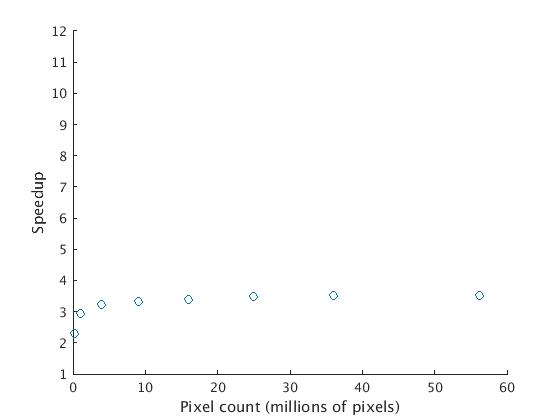
\includegraphics[width=0.45\textwidth]{separable_convolution_speedup_graph.jpg}
	\caption{Visualization of separable convolution speedup versus pixel count}
    \label{separable-convolution-speedup-graph}
\end{figure}

\subsection{Non-maximum Suppression and Selective Thresholding}
As discussed previously, our CUDA implementation of non-maximum suppression and selective thresholding is split into two parallel tasks that run one after the other: computation of the gradient magnitude and angle, followed by the actual edge selection algorithm. The computations for the speedup numbers below reflect the full procedure of calculating the gradient's magnitude and angle, selecting edges, and finally copying the results to host memory.
\begin{table}[H]
	\small
	\centering
	\caption{Speedup of Non-maximum Suppression and Selective Thresholding}
	\label{non-maximum-suppression-selective-thresholding-speedup}
	\begin{tabular}{llllll}
	 Image dimensions & CPU time (s) & GPU time (s) & Speedup \\
	 $100 \times 100$ & $0.033848$ & $0.000347$ & $97.544669$ \\
	 $500 \times 500$ & $0.070105$ & $0.006773$ & $10.350657$ \\
	 $1000 \times 1000$ & $0.213390$ & $0.022899$ & $9.318748$ \\
	 $2000 \times 2000$ & $0.616050$ & $0.078498$ & $7.847971$ \\
	 $3000 \times 3000$ & $1.114336$ & $0.160118$ & $6.959467$ \\
	 $4000 \times 4000$ & $1.627116$ & $0.265466$ & $6.129282$ \\
	 $5000 \times 5000$ & $2.215267$ & $0.388015$ & $5.709230$ \\
	 $6000 \times 6000$ & $2.764201$ & $0.528509$ & $5.230187$ \\
	\end{tabular}
\end{table}
\begin{figure}[h]
	\centering
	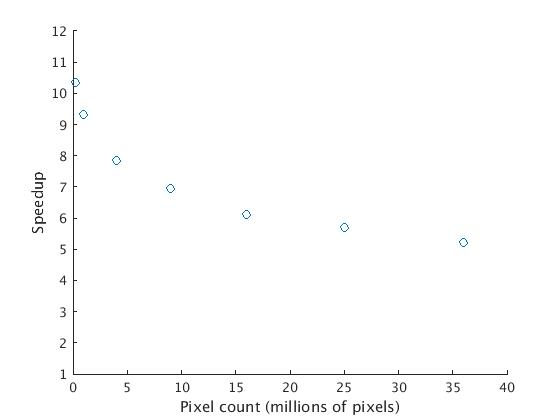
\includegraphics[width=0.45\textwidth]{non_maximum_suppression_selective_thresholding_speedup_graph.jpg}
	\caption{Visualization of non-maximum suppression and selective thresholding speedup versus pixel count}
    \label{non-maximum-suppression-selective-thresholding-speedup-graph}
\end{figure}

\subsection{Thresholded Difference Density Matrix and Motion Area Estimation}
The below results reflect the speedup in the complete procedure of calculating the difference matrix $\boldsymbol{D}_0$, determining the thresholded difference matrix $\boldsymbol{D}$, building a difference density matrix $\boldsymbol{D}'$, and finally generating an image representing the estimated motion area.
\begin{table}[H]
	\small
	\centering
	\caption{Speedup of Motion Area Estimation}
	\label{motion-area-speedup}
	\begin{tabular}{llllll}
	 Image dimensions & CPU time (s) & GPU time (s) & Speedup \\
	 $100 \times 100$ & $0.008400$ & $0.001652$ & $5.084746$ \\
	 $500 \times 500$ & $0.214381$ & $0.027413$ & $7.820414$ \\
	 $1000 \times 1000$ & $0.866711$ & $0.097432$ & $8.895548$ \\
	 $2000 \times 2000$ & $3.468732$ & $0.388721$ & $8.923449$ \\
	 $3000 \times 3000$ & $8.320342$ & $0.871464$ & $9.547545$ \\
	 $4000 \times 4000$ & $14.841659$ & $1.569390$ & $9.456960$ \\
	 $5000 \times 5000$ & $22.094181$ & $2.546088$ & $8.677697$ \\
	 $6000 \times 6000$ & $31.911879$ & $3.624211$ & $8.805193$ \\
	 $7500 \times 7500$ & $55.772766$ & $13.077988$ & $4.264629$ \\
	\end{tabular}
\end{table}
\begin{figure}[h]
	\centering
	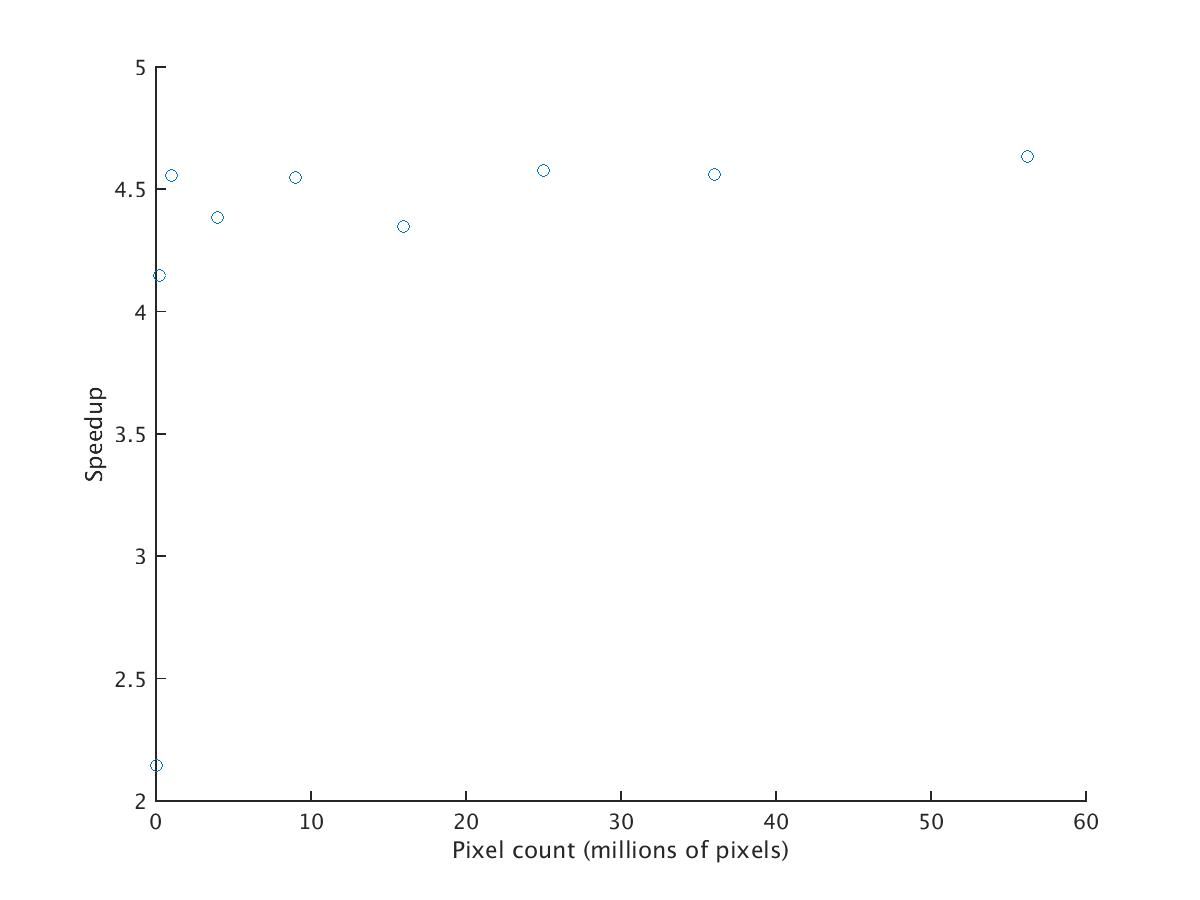
\includegraphics[width=0.45\textwidth]{motion_area_estimation_speedup_graph.jpg}
	\caption{Visualization of motion area estimation speedup versus pixel count}
    \label{motion-area-estimation-speedup-graph}
\end{figure}

\subsection{Facial Recognition}
The below results reflect the speedup achieved using OpenCV's object detection framework.
\begin{table}[H]
	\small
	\centering
	\caption{Speedup of Facial Recognition}
	\label{facial-recognition-speedup}
	\begin{tabular}{llllll}
	 Image dimensions & CPU time (s) & GPU time (s) & Speedup \\
	 $100 \times 100$ & $0.067883$ & $0.061132$ & $1.110433$ \\
	 $500 \times 500$ & $0.226192$ & $0.094812$ & $2.385690$ \\
	 $1000 \times 1000$ & $0.811302$ & $0.199005$ & $4.076792$ \\
	 $2000 \times 2000$ & $2.849201$ & $0.562820$ & $5.062366$ \\
	 $3000 \times 3000$ & $6.236422$ & $1.218879$ & $5.116523$ \\
	 $4000 \times 4000$ & $10.794892$ & $2.142449$ & $5.038576$ \\
	\end{tabular}
\end{table}
\begin{figure}[h]
	\centering
	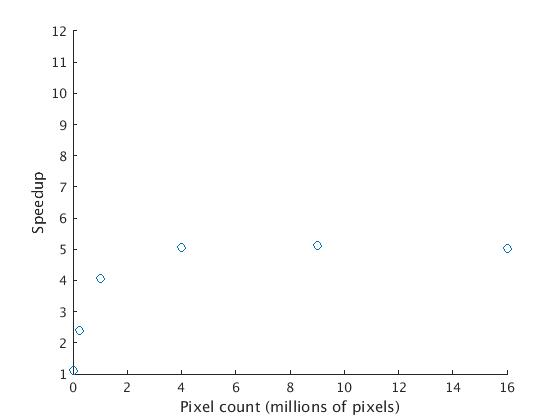
\includegraphics[width=0.45\textwidth]{facial_recognition_speedup_graph.jpg}
	\caption{Visualization of facial recognition speedup versus pixel count}
    \label{facial-recognition-speedup-graph}
\end{figure}

\subsection{Real-time Motion Detection Performance}
Our real-time motion detection implementation continuously repeats the following procedure in an infinite loop:
\begin{enumerate}
	\item Read two frames $\boldsymbol{F}_1$ and $\boldsymbol{F}_2$ from the camera in succession
	\item Apply a Gaussian low-pass filter of kernel size $k = 3$ to both frames
	\item Apply a Sobel edge filter in both directions
	\item Calculate the edges $\boldsymbol{E}_1$ and $\boldsymbol{E}_2$ from the image with non-maximum suppression and selective thresholding
	\item Calculate the difference matrix $\boldsymbol{D}$ and difference density matrix $\boldsymbol{D}'$
	\item Draw an image representing the portions of the image with motion
	\item Update a live preview of $\boldsymbol{F}_1$, $\boldsymbol{E}_1$, $\boldsymbol{D}'$, and the motion area estimate
\end{enumerate}
Table \ref{real-time-fps-statistics} shows basic statistics on the frame rate results achieved on a $640 \times 480$ continuous video stream, running on the same hardware as the benchmarks in the previous section. The frame rate was evaluated on a 10-second video stream in a well-lit environment with motion of a moderate number of edge pixels ($< 10\%$ of the total number of pixels in the frame) in front of the camera. All procedures (as described in this paper) were executed in parallel on the GPU.
\begin{table}[H]
	\small
	\centering
	\caption{Real-time Frame Rate Statistics}
	\label{real-time-fps-statistics}
	\begin{tabular}{ll}
	 Average FPS & $11.01$ \\
	 Median FPS & $10.72$ \\
	 Min FPS & $9.68$ \\
	 Max FPS & $12.02$ \\
	 Standard deviation & $0.37$ \\
	\end{tabular}
\end{table}

\section{Conclusion}
\label{conclusion}
Our CUDA implementation of both the edge detection and motion detection algorithms demonstrate that parallelized, GPU computation results in significant speedups compared to a serial, CPU implementation. In all benchmarked cases (separable convolution with a Gaussian filter, edge detection via non-maximum suppression and selective thresholding, and motion area estimation from a difference density map), we find that the GPU implementation, running on a mid-range graphics card, demonstrated anywhere between a 1.5x to 4.6x speedup over a relatively high-performance, overclocked CPU. Furthermore, we observe a similar speedup trend when comparing existing OpenCV CPU and GPU CUDA implementations of HAAR-based facial recognition. In all cases, we find that the speedup asymptotically approaches a general range as the input size increases.
\par It is important to note the edge case for the separable convolution algorithm on images of small input sizes (namely, near the dimensions $100 \times 100$, or $10000$ total pixels). For this case, we observe a remarkably underwhelming speedup ratio of 0.001521, suggesting that a CPU implementation is nearly 700 times as fast as a GPU implementation (Table \ref{separable-convolution-speedup}). We speculate that, because the input size is very small (especially in comparison to the larger versions of the same image, which exceed 55 million total pixels in size), the additional overhead caused by launching the GPU kernel (e.g. allocating device memory, copying the host arrays onto the device, and copying the device arrays back to the host following completion of the computation) causes the GPU code to take much longer to run than the more directly implemented CPU code. This reasoning is backed by the fact that, at a $250000$ total pixel count (a $500 \times 500$ image), the speedup ($2.306766$) is still much lower than the asymptotic value it approaches as the pixel count exceeds about 1 million ($2.932381$).
\par However, an opposite trend appears to be in play for the speedup of the non-maximum suppression and selective thresholding algorithm (Table \ref{non-maximum-suppression-selective-thresholding-speedup}), where we observe a high speedup for low input sizes and a lower speedup for high input sizes. We speculate that this is most likely due to the overhead of running two separate parallel tasks in sequence, both of which require the same amount of memory. As a result of our implementation, not only does a large input size result in a greater percentage of the time that any thread is idle, but it also doubles the total memory footprint of the algorithm. This is evident from the significantly higher memory consumption of this procedure compared to the others; an input size of 36 million pixels nearly maxes out the 2 GB of available GPU memory, while the other algorithms consume no more than a few hundred megabytes on the largest benchmarking image we use. Despite this trend, the speedup is still greater than 1 for large input sizes, suggesting that a GPU implementation is still consistently faster than its CPU counterpart.
\par While we were successful in exploiting the parallel architecture of GPUs to achieve significant speedups, there are still many areas in GPU computation we have yet to explore. Our CUDA code for the edge detection and motion detection are direct implementations of the algorithms (albeit parallelized on each pixel in the image). We did not attempt any degree of memory optimization beyond ensuring that no memory leaks occur on either the host or device when running the real-time program. We also did not attempt to minimize the amount of time any given GPU thread is idle; this delay (after a particular thread has finished its computation task but has not yet been assigned another computation task) is most likely the largest bottleneck in our parallel performance. Future improvements to our existing work would lie primarily in optimizing these parameters, thereby increasing performance.
\par A future goal is exploring multi-GPU computation. Our implementation, through parallelized, is optimized to run only on a single GPU. Multi-GPU computation would add another layer of parallelism that could theoretically increase the throughput of our computation by the number of GPUs across which the work is divided. NVIDIA's existing multi-GPU computational platform is marketed as Scalable Link Interface (SLI), allowing for the simultaneous use of 2 to 4 GPUs to render real-time graphics. In context of the work we present here, a possible future goal is to explore the performance and memory efficiency gain from Split Frame Rendering (SFR), by allowing each of our parallel algorithms to operate simultaneously on a division of the input image; or Alternate Frame Rendering (AFR), to allow for the simultaneous computation on multiple sets of 2 frames.

\section*{Source Code}
The full source code for this project, including CUDA, Python, and MATLAB implementations of all of our algorithms, is open sourced and available at \texttt{github.com/LINKIWI/cuda-computer-vision}.

\section*{Authors}
\begin{itemize}
	\item \textbf{Emilio Del Vechhio}, Electrical and Computer Engineering `18
	\item \textbf{Kevin Lin}, Electrical and Computer Engineering `18
	\item \textbf{Senthil Natarajan}, Electrical and Computer Engineering `17
\end{itemize}

\section*{Acknowledgments}
\begin{itemize}
	\item \textbf{CJ Barberan}, ECE Ph.D. student, Rice University---\textit{for mentoring the entire team in the conception, development, and extensive debugging of our project}.
	\item \textbf{Richard Baraniuk}, Victor E. Cameron Professor of ECE, Rice University---\textit{for his Fall 2015 instruction of the signal processing course that inspired this project}.
\end{itemize}

\end{document}